% =============================================================================
% Section 4: Results
% =============================================================================
\section{Results}
\label{sec:results}

This section presents findings from 918 experimental runs: 648 final training runs (9~models $\times$ 12~assets $\times$ 2~horizons $\times$ 3~seeds) plus 270 HPO trials.  Results are organised by the four hypotheses from Section~\ref{sec:hypotheses}.  All claims reference specific tables or figures; mechanistic interpretation is deferred to Section~\ref{sec:discussion}.

% --------------------------------------------------------------------------
\subsection{Global Performance Rankings}
\label{sec:global_rankings}

Table~\ref{tab:global_leaderboard} presents the global leaderboard, ranking \nmodels models across four architectural families by mean \rmse rank across all \nassets assets and both horizons (24~evaluation points per model).  Three distinct performance tiers emerge:

\begin{itemize}[nosep]
  \item \textbf{Top tier:} \moderntcn (CNN; mean rank 1.333, median 1.0) and \patchtst (Transformer; mean rank 2.000, median 2.0).
  \item \textbf{Middle tier:} \itransformer (3.667), \timexer (4.292), \dlinear (4.958), and \nhits (5.250), spanning the Transformer and MLP / Linear families.
  \item \textbf{Bottom tier:} \timesnet (7.708), \autoformer (7.833), and \lstm (7.958).
\end{itemize}

The separation between tiers is substantial: the gap between the top tier (ranks 1--2) and bottom tier (ranks 7--9) spans more than 5.5 rank positions, and performance does not correlate uniformly with model family. Both the top and bottom tiers contain CNN and Transformer-based architectures, suggesting that specific implementation details (e.g., patching, large-kernel convolutions) matter more than broad architectural classes.

% =============================================================================
% Table 6: Global Leaderboard
% =============================================================================
\begin{table}[htbp]
  \centering
  \caption{Global model ranking aggregated across all 12 assets and both
    horizons ($h\in\{4,24\}$), categorised by architectural family. Each
    (asset, horizon) pair contributes one rank based on mean \rmse over
    three seeds.  Mean and median ranks are computed over 24 evaluation slots.
    Win~Count indicates the number of slots in which a model achieved rank~1.
    Bold marks the best value per column.}
  \label{tab:global_leaderboard}
  \setlength{\tabcolsep}{6pt}%
  \begin{tabular}{%
    l%
    l%                    Family
    S[table-format=1.3]%  Mean Rank
    S[table-format=1.1]%  Median Rank
    l%                    Wins
  }
    \toprule
    \textbf{Model}
      & \textbf{Family}
      & {\textbf{Mean Rank}}
      & {\textbf{Median Rank}}
      & \textbf{Wins (of 24)} \\
    \midrule
    \textbf{\moderntcn} & CNN           & \bfseries 1.333 & \bfseries 1.0 & \textbf{18~(75.0\%)} \\
    \patchtst           & Transformer   & 2.000           & 2.0           & 3~(12.5\%)            \\
    \itransformer       & Transformer   & 3.667           & 3.0           & 0                     \\
    \timexer            & Transformer   & 4.292           & 4.0           & 0                     \\
    \dlinear            & MLP / Linear  & 4.958           & 5.0           & 0                     \\
    \nhits              & MLP / Linear  & 5.250           & 6.0           & 3~(12.5\%)            \\
    \timesnet           & CNN           & 7.708           & 8.0           & 0                     \\
    \autoformer         & Transformer   & 7.833           & 8.0           & 0                     \\
    \lstm               & RNN           & 7.958           & 9.0           & 0                     \\
    \bottomrule
  \end{tabular}
\end{table}


In terms of win counts, \moderntcn achieves the lowest \rmse on 18 of 24~evaluation points (75.0\% win rate), while \nhits and \patchtst each win 3~points (12.5\%).  No other architecture achieves a single first-place finish.

Table~\ref{tab:per_asset_best_models} disaggregates these wins by asset and horizon. \moderntcn's dominance is concentrated in forex and equity indices (16 of 16~wins), while its cryptocurrency record is more contested: \nhits wins on ETH/USDT (both horizons) and ADA/USDT ($\hfour$), and \patchtst wins on BTC/USDT ($\hfour$; $\rmse = 731.05$ vs.\ \moderntcn's $731.63$, $\Delta = 0.08\%$) and ADA/USDT ($\htwentyfour$).  Notably, no model other than \moderntcn achieves the lowest \rmse on any forex or equity index asset at $\htwentyfour$, underscoring its superior long-horizon generalisation outside the cryptocurrency domain.

% =============================================================================
% Table 12: Per-Asset Best Model Matrix
% =============================================================================
\begin{table}[htbp]
  \centering
  \begin{threeparttable}
  \caption{Best-performing model per asset and horizon, determined by lowest
    mean \rmse across three seeds.  \moderntcn achieves the lowest \rmse
    on 18 of 24~evaluation points (75\%); \nhits wins on 3~points
    (all in cryptocurrency); \patchtst wins on 3~points (one crypto,
    one crypto, one forex).  Bold highlights non-\moderntcn winners,
    revealing niche asset-specific advantages.}
  \label{tab:per_asset_best_models}
  \setlength{\tabcolsep}{7pt}%
  \begin{tabular}{l l l l}
    \toprule
    \textbf{Category} & \textbf{Asset}
      & \textbf{Best at $\hfour$}
      & \textbf{Best at $\htwentyfour$} \\
    \midrule
    \multirow{4}{*}{Crypto}
      & BTC/USDT    & \textbf{\patchtst}  & \moderntcn          \\
      & ETH/USDT    & \textbf{\nhits}     & \textbf{\nhits}     \\
      & BNB/USDT    & \moderntcn          & \moderntcn          \\
      & ADA/USDT    & \textbf{\nhits}     & \textbf{\patchtst}  \\
    \addlinespace
    \multirow{4}{*}{Forex}
      & EUR/USD     & \moderntcn          & \moderntcn          \\
      & USD/JPY     & \moderntcn          & \moderntcn          \\
      & GBP/USD     & \textbf{\patchtst}  & \moderntcn          \\
      & AUD/USD     & \moderntcn          & \moderntcn          \\
    \addlinespace
    \multirow{4}{*}{Indices}
      & DAX         & \moderntcn          & \moderntcn          \\
      & Dow Jones   & \moderntcn          & \moderntcn          \\
      & S\&P~500    & \moderntcn          & \moderntcn          \\
      & NASDAQ~100  & \moderntcn          & \moderntcn          \\
    \midrule
    \multicolumn{2}{l}{\textbf{Win count summary}}
      & \multicolumn{2}{l}{\moderntcn: 18\quad \nhits: 3\quad \patchtst: 3} \\
    \bottomrule
  \end{tabular}
  \begin{tablenotes}[flushleft]\footnotesize
    \item \nhits wins exclusively on lower-capitalisation cryptocurrency
      assets (ETH/USDT, ADA/USDT), suggesting that its hierarchical
      multi-rate pooling is particularly suited to the high-frequency,
      multi-scale volatility structure of altcoin markets.
    \item \patchtst wins at $\hfour$ on BTC/USDT ($\rmse = 731.05$
      vs.\ \moderntcn's $731.63$; $\Delta = 0.08\%$) and on
      GBP/USD, but cedes to \moderntcn at $\htwentyfour$ in both cases.
    \item No model other than \moderntcn wins on any forex or equity index
      asset at $\htwentyfour$, underscoring its superior long-horizon
      generalisation.
  \end{tablenotes}
  \end{threeparttable}
\end{table}


Figure~\ref{fig:global_heatmap} displays the \rmse heatmap across all evaluation points.  The body panel excludes \lstm to reveal finer distinctions among the eight modern architectures (the all-models variant appears in Appendix~\ref{sec:app_dual_plots}).  \moderntcn and \patchtst consistently occupy the lowest-error cells.  Figure~\ref{fig:global_rank_comparison} presents the rank distribution, confirming the three-tier structure.

\begin{figure}[htbp]
  \centering
  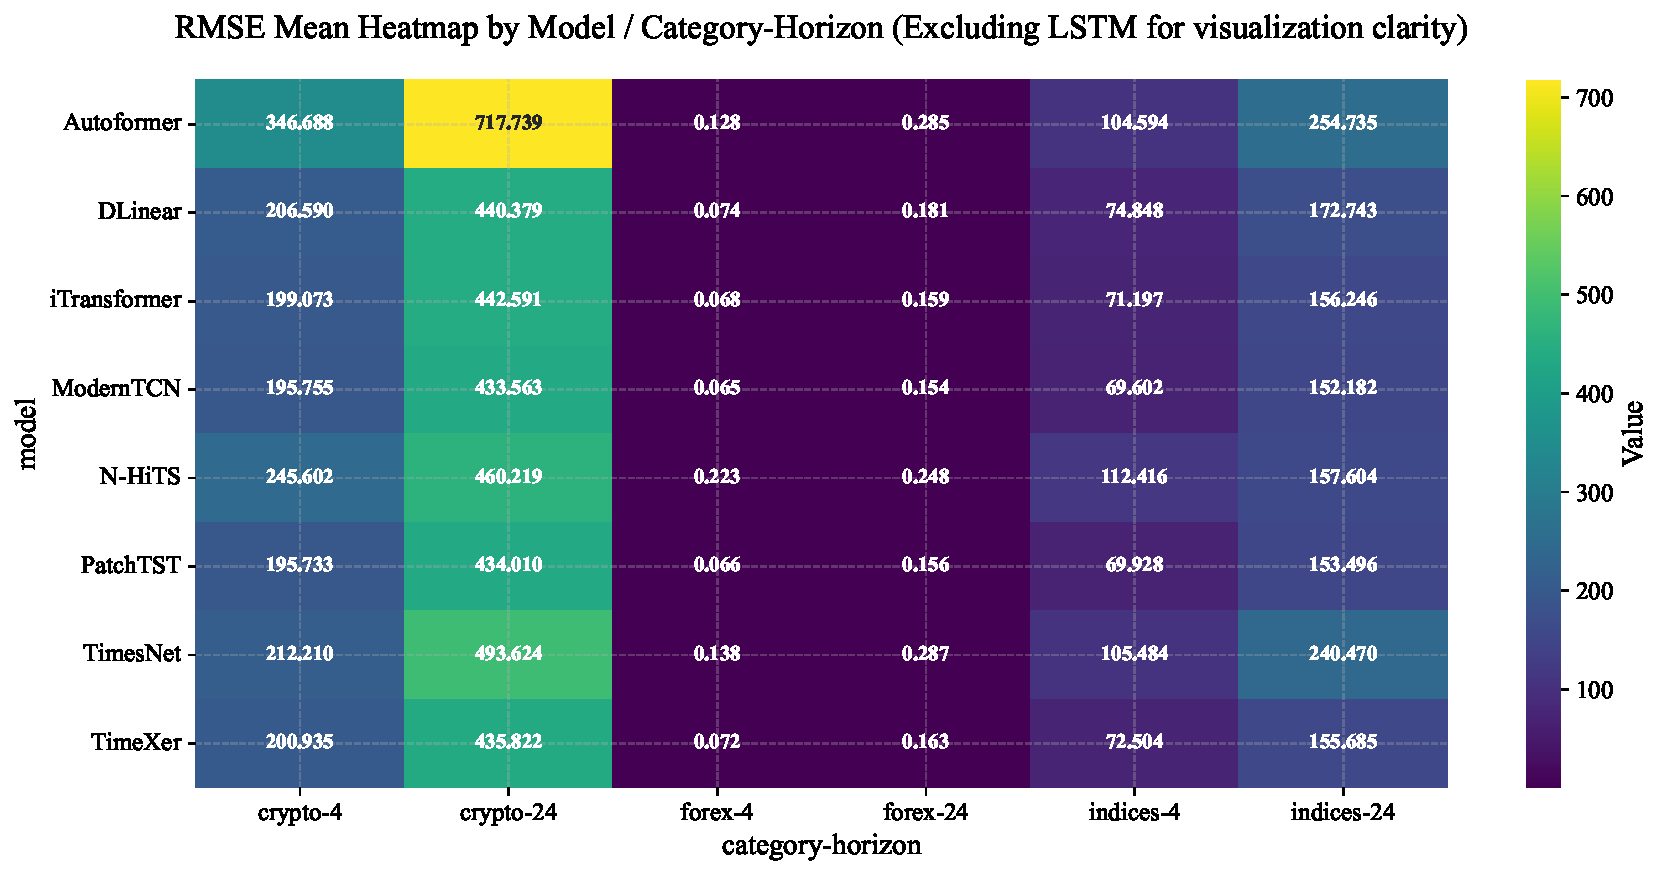
\includegraphics[width=0.85\textwidth]{figures/03_global_performance/global_metric_heatmap_no_lstm.pdf}
  \caption{Global \rmse heatmap across eight modern architectures and 24 evaluation points (12~assets $\times$ 2~horizons).  Lighter cells indicate lower error.  \moderntcn and \patchtst consistently achieve the lowest \rmse values across all asset--horizon combinations.  \lstm is excluded for visual clarity; the full nine-model variant is provided in Appendix~\ref{sec:app_dual_plots}, Figure~\ref{fig:app_global_heatmap_all}.  Values represent mean \rmse across three seeds.}
  \label{fig:global_heatmap}
\end{figure}

\begin{figure}[htbp]
  \centering
  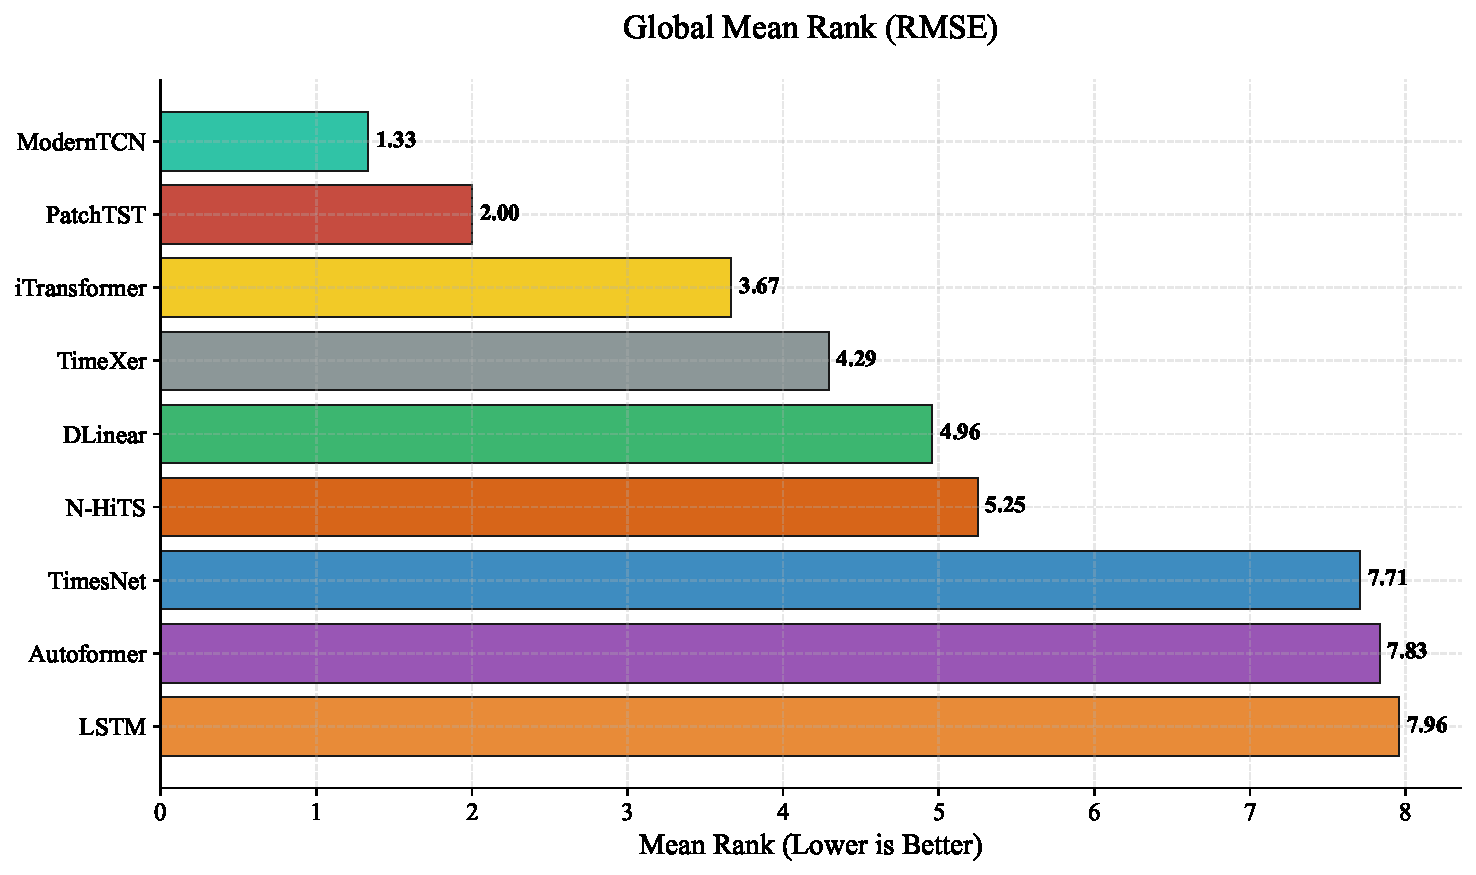
\includegraphics[width=0.7\textwidth]{figures/03_global_performance/global_rank_comparison.pdf}
  \caption{Global mean rank comparison across 24 evaluation points (12~assets $\times$ 2~horizons).  Lower values indicate better performance.  Three distinct tiers are visible: \moderntcn and \patchtst (ranks 1--2), a middle group of four models (ranks 3--6), and a bottom group comprising \timesnet, \autoformer, and \lstm (ranks 7--9).  Error bars represent rank standard deviation across evaluation points.}
  \label{fig:global_rank_comparison}
\end{figure}

% --------------------------------------------------------------------------
\subsection{Category-Level Analysis}
\label{sec:category_analysis}

Table~\ref{tab:category_metrics} reports category-level aggregated \rmse and \mae for each model, providing the asset-class dimension of H1.  Error magnitudes differ by several orders of magnitude across categories due to underlying price scales, but relative model ordering is preserved.



% siunitx setup (CRITICAL)
\sisetup{
  detect-weight          = true,
  text-series-to-math    = true,
  table-number-alignment = center
}

% =============================================================================
% Table 7: Category-Level Metrics (RMSE and MAE, averaged over assets and seeds)
% =============================================================================
\begin{table}[htbp]
  \centering
  \caption{Category-level mean \rmse and \mae averaged across all assets within
    each category and across both horizons ($h\in\{4,24\}$).  Values are
    aggregated over 4~assets $\times$ 2~horizons $\times$ 3~seeds.  Bold
    marks the best (lowest) value per category and metric.  \lstm is
    included for completeness but excluded from ranking discussions
    due to convergence failures.}
  \label{tab:category_metrics}
  \footnotesize
  \setlength{\tabcolsep}{7pt}%
  \resizebox{\textwidth}{!}{%
  \begin{tabular}{%
    l%
    S[table-format=4.2, round-mode=places, round-precision=2] @{\hspace{2pt}}
    S[table-format=4.2, round-mode=places, round-precision=2]%  Crypto
    S[table-format=1.4, round-mode=places, round-precision=4] @{\hspace{2pt}}
    S[table-format=1.4, round-mode=places, round-precision=4]%  Forex
    S[table-format=4.2, round-mode=places, round-precision=2] @{\hspace{2pt}}
    S[table-format=4.2, round-mode=places, round-precision=2]%  Indices
  }
    \toprule
    & \multicolumn{2}{c}{\textbf{Crypto}}
    & \multicolumn{2}{c}{\textbf{Forex}}
    & \multicolumn{2}{c}{\textbf{Indices}} \\
    \cmidrule(lr){2-3} \cmidrule(lr){4-5} \cmidrule(lr){6-7}
    \textbf{Model}
      & {\rmse} & {\mae}
      & {\rmse} & {\mae}
      & {\rmse} & {\mae} \\
    \midrule
    \autoformer         & 532.21  & 393.83  & 0.2068 & 0.1551 & 179.66  & 136.24  \\
    \dlinear            & 323.48  & 220.87  & 0.1279 & 0.0940 & 123.80  &  90.67  \\
    \itransformer       & 320.83  & 217.99  & 0.1136 & 0.0785 & 113.72  &  79.13  \\
    \lstm               & 2398.94 & 2041.58 & 3.6679 & 3.5858 & 1548.56 & 1478.21 \\
    \textbf{\moderntcn} 
                        & \bfseries 314.66 & \bfseries 211.14 
                        & \bfseries 0.1098 & \bfseries 0.0750 
                        & \bfseries 110.89 & \bfseries 76.09 \\
    \nhits              & 352.91  & 255.77  & 0.2356 & 0.1977 & 135.01  & 101.04  \\
    \patchtst           & 314.87  & 211.70  & 0.1108 & 0.0761 & 111.71  &  77.04  \\
    \timesnet           & 352.92  & 249.41  & 0.2127 & 0.1596 & 172.98  & 131.61  \\
    \timexer            & 318.38  & 215.24  & 0.1174 & 0.0815 & 114.09  &  79.19  \\
    \bottomrule
  \end{tabular}%
  }%
\end{table}

\paragraph{Cryptocurrency.}
\moderntcn achieves the lowest mean \rmse (314.66), closely followed by \patchtst (314.87; $\Delta = 0.07\%$) and \timexer (318.38).  \itransformer (320.83) and \dlinear (323.48) are competitive within a 3\% range of the leader.  \lstm exhibits errors approximately $7.6\times$ higher than the best model (2{,}398.94), reflecting fundamental convergence difficulties under the standard training protocol.  \nhits (352.91), \autoformer (532.21), and \timesnet (352.92) form the lower-performing group.

\paragraph{Forex.}
\moderntcn leads (mean \rmse 0.1098), followed by \patchtst (0.1108; $\Delta = 0.9\%$) and \itransformer (0.1136).  \timexer (0.1174) and \dlinear (0.1279) remain competitive on an absolute scale.  \lstm (3.668) is approximately $33\times$ worse than the leader, while \nhits (0.2356), \autoformer (0.2068), and \timesnet (0.2127) form the lower tier.

\paragraph{Equity indices.}
\moderntcn achieves the lowest \rmse (110.89), with \patchtst (111.71; $\Delta = 0.7\%$), \itransformer (113.72), and \timexer (114.09) in close succession.  \dlinear (123.80) and \nhits (135.01) are moderately higher.  \timesnet (172.98), \autoformer (179.67), and \lstm (1{,}548.56) trail substantially.

\paragraph{Cross-category ranking consistency.}
Across all three categories, \moderntcn and \patchtst consistently occupy the top two positions (Figure~\ref{fig:category_boxplot}).  This consistency is confirmed by the \rmse--\mae concordance in Figure~\ref{fig:category_scatter}: near-perfect linear correlation between the two error metrics shows that rankings are robust to metric choice.  Category dendrograms and per-category performance matrices appear in Appendix~\ref{sec:app_category_rankings} (Figures~\ref{fig:app_category_hierarchical_rankings} and~\ref{fig:app_category_performance_matrices}); \moderntcn and \patchtst cluster at the top of every dendrogram.

\begin{figure}[htbp]
  \centering
  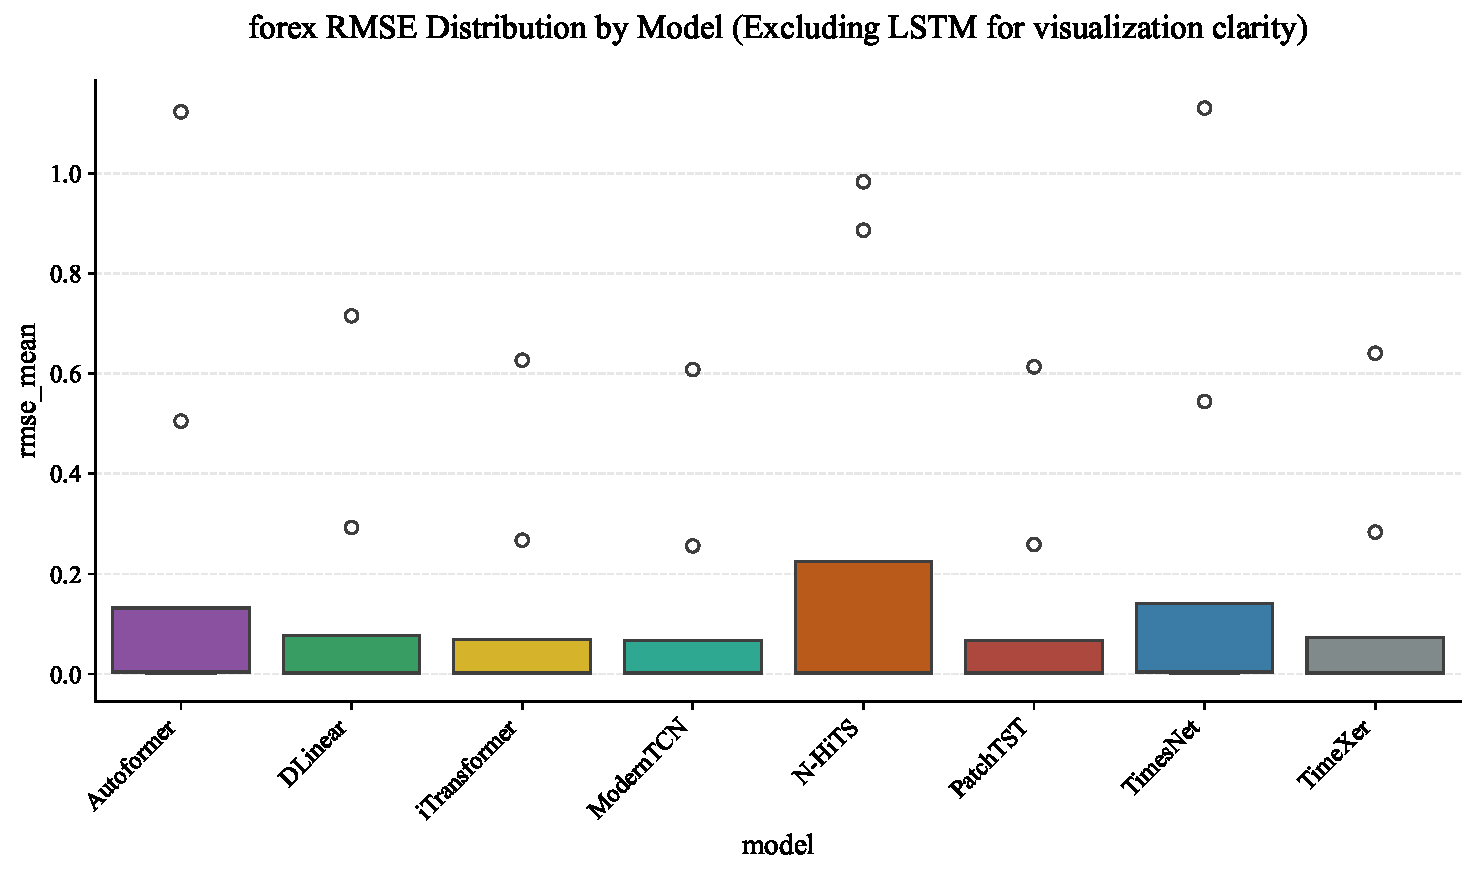
\includegraphics[width=0.75\textwidth]{figures/04_category_analysis/category_rank_boxplot_no_lstm.pdf}
  \caption{Category-level rank distributions across assets within each category, excluding \lstm for visual clarity.  \moderntcn exhibits the tightest rank distribution (consistently rank~1 across all categories), indicating stable cross-asset performance.  The full nine-model variant is provided in Appendix~\ref{sec:app_dual_plots}.  Boxes show interquartile range; whiskers extend to the most extreme rank observed.}
  \label{fig:category_boxplot}
\end{figure}

\begin{figure}[htbp]
  \centering
  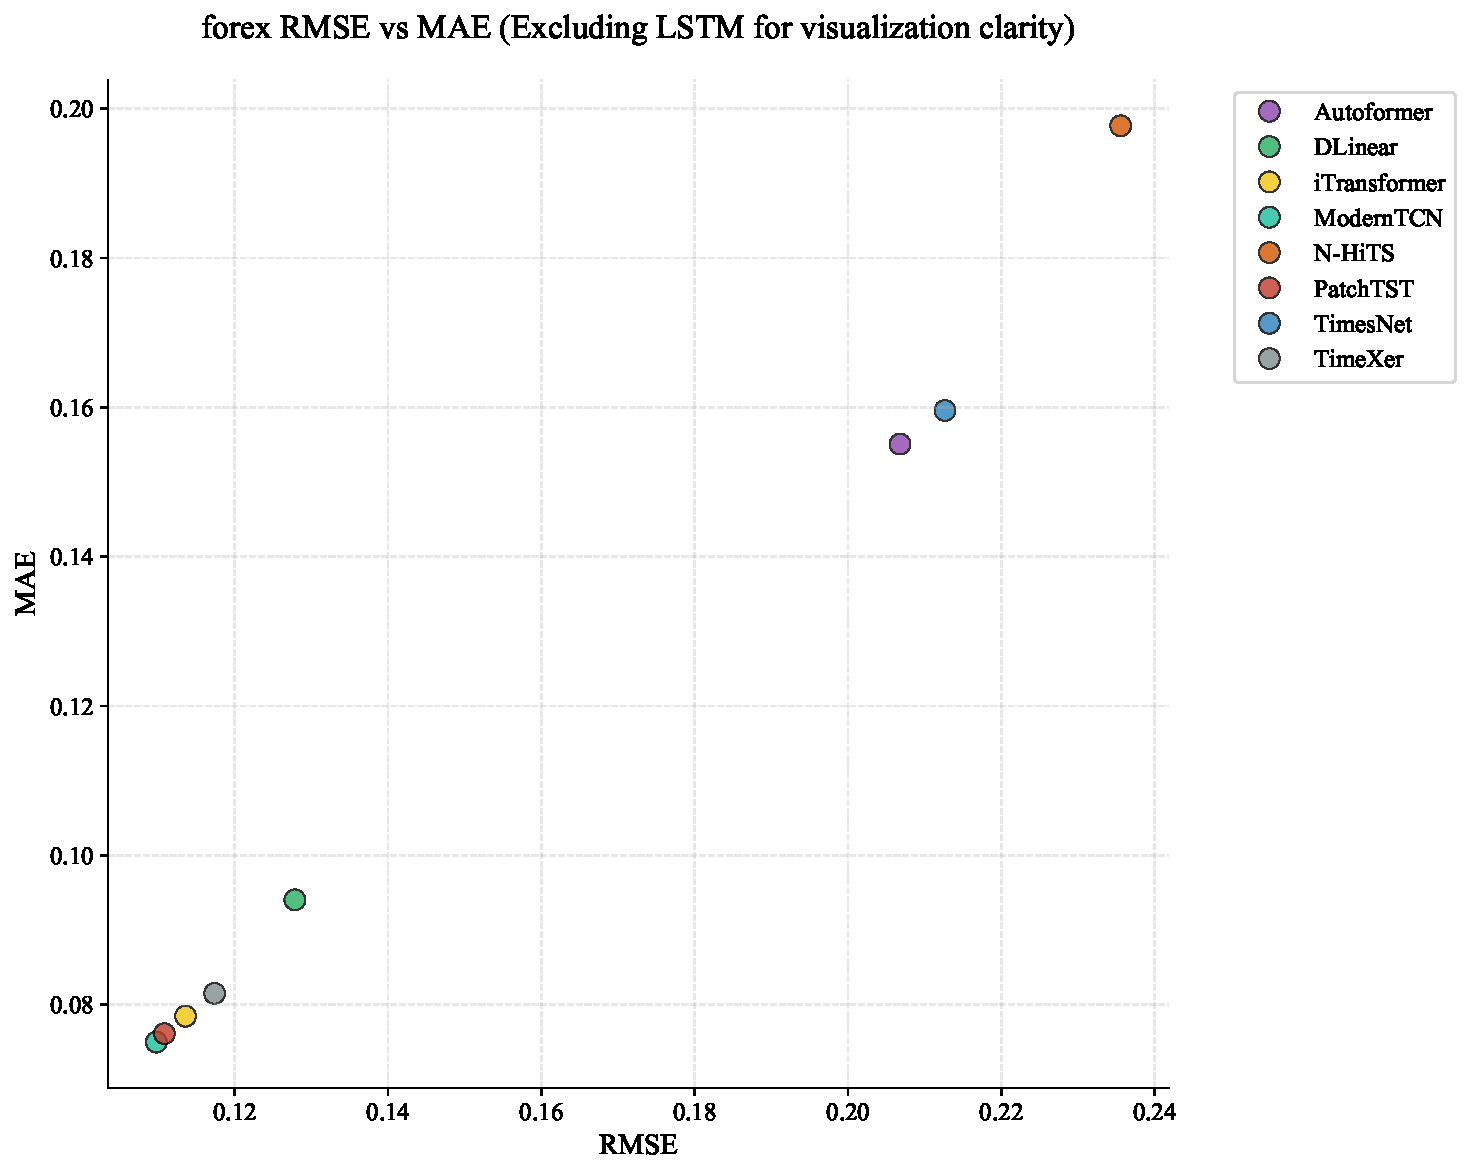
\includegraphics[width=0.75\textwidth]{figures/04_category_analysis/category_scatter_rmse_mae_no_lstm.pdf}
  \caption{Category-level \rmse vs.\ \mae scatter plot for eight modern architectures.  Each point represents one model's mean error within a category.  The near-perfect linear correlation ($R^2 > 0.99$) confirms that model rankings are consistent across the two error metrics, indicating that findings based on \rmse generalise to \mae.  The full nine-model variant is provided in Appendix~\ref{sec:app_dual_plots}.}
  \label{fig:category_scatter}
\end{figure}


% --------------------------------------------------------------------------
\subsection{Cross-Horizon Degradation}
\label{sec:horizon_degradation}

Table~\ref{tab:horizon_degradation_btc} presents \rmse at $\hfour$ and $\htwentyfour$ for each representative asset (BTC/USDT, EUR/USD, Dow Jones), along with the percentage degradation ($\Delta\% = 100 \times (\text{RMSE}_{h=24} - \text{RMSE}_{h=4}) / \text{RMSE}_{h=4}$).  Table~\ref{tab:horizon_ranking_shift} provides the corresponding rank shift $\Delta = r_{24} - r_4$ for each model, isolating relative ordering changes from absolute error magnitudes.

% =============================================================================
% Table 8: Horizon Degradation (Representative Assets)
% Three sub-tables, one per representative asset, set side by side.
% =============================================================================

% ---- BTC/USDT ---------------------------------------------------------------
\begin{table}[htbp]
  \centering
  \caption{Horizon degradation for \textbf{BTC/USDT} (top), \textbf{EUR/USD}
    (middle), and \textbf{Dow Jones} (bottom).  \rmse values are three-seed
    means.  $\Delta\%$ denotes the relative \rmse increase from $h{=}4$ to
    $h{=}24$: $\Delta\% = 100\times(\mathrm{RMSE}_{24} -
    \mathrm{RMSE}_{4})/\mathrm{RMSE}_{4}$.  Bold marks the model with the
    lowest \rmse at $h{=}24$ across all nine architectures.}
  \label{tab:horizon_degradation_btc}
  \setlength{\tabcolsep}{9pt}%
  \begin{tabular}{l
    S[table-format=5.2, round-precision=2]
    S[table-format=5.2, round-precision=2]
    S[table-format=3.2, round-precision=2]}
    \toprule
    \textbf{Model}
      & {\rmse, $h{=}4$}
      & {\rmse, $h{=}24$}
      & {$\Delta\%$} \\
    \midrule
    \autoformer   & 1284.9  & 2670.0  & 107.8 \\
    \dlinear      &  772.0  & 1644.1  & 113.0 \\
    \itransformer &  743.5  & 1651.3  & 122.1 \\
    \lstm         & 8029.9  & 10878.7 &  35.5 \\
    \moderntcn    &  731.6  & \bfseries 1617.4  & 121.1 \\
    \nhits        &  930.5  & 1724.5  &  85.3 \\
    \patchtst     &  731.1  & 1619.1  & 121.5 \\
    \timesnet     &  793.6  & 1840.4  & 131.9 \\
    \timexer      &  750.3  & 1624.9  & 116.6 \\
    \bottomrule
  \end{tabular}
\end{table}

% ---- EUR/USD ----------------------------------------------------------------
\begin{table}[htbp]
  \centering
  \caption{Horizon degradation for \textbf{EUR/USD}.  \rmse values are
    three-seed means.  $\Delta\%$ defined as in
    Table~\ref{tab:horizon_degradation_btc}.}
  \label{tab:horizon_degradation_eurusd}
  \setlength{\tabcolsep}{9pt}%
  \begin{tabular}{l
    S[table-format=1.2, round-precision=2]
    S[table-format=1.2, round-precision=2]
    S[table-format=3.2, round-precision=2]}
    \toprule
    \textbf{Model}
      & {\rmse, $h{=}4$}
      & {\rmse, $h{=}24$}
      & {$\Delta\%$} \\
    \midrule
    \autoformer   & 0.00284 & 0.00626 & 120.3 \\
    \dlinear      & 0.00159 & 0.00347 & 118.5 \\
    \itransformer & 0.00156 & 0.00345 & 121.0 \\
    \lstm         & 0.00179 & 0.00364 & 102.6 \\
    \moderntcn    & 0.00152 & \bfseries 0.00338 & 121.4 \\
    \nhits        & 0.00170 & 0.00353 & 107.4 \\
    \patchtst     & 0.00153 & 0.00344 & 124.9 \\
    \timesnet     & 0.00298 & 0.00627 & 110.3 \\
    \timexer      & 0.00161 & 0.00349 & 116.7 \\
    \bottomrule
  \end{tabular}
\end{table}

% ---- Dow Jones --------------------------------------------------------------
\begin{table}[htbp]
  \centering
  \caption{Horizon degradation for \textbf{Dow Jones}.  \rmse values are
    three-seed means.  $\Delta\%$ defined as in
    Table~\ref{tab:horizon_degradation_btc}.}
  \label{tab:horizon_degradation_usa30}
  \setlength{\tabcolsep}{9pt}%
  \begin{tabular}{l
    S[table-format=4.2, round-precision=2]
    S[table-format=4.2, round-precision=2]
    S[table-format=3.2, round-precision=2]}
    \toprule
    \textbf{Model}
      & {\rmse, $h{=}4$}
      & {\rmse, $h{=}24$}
      & {$\Delta\%$} \\
    \midrule
    \autoformer   &  160.7 &  410.7 & 155.6 \\
    \dlinear      &  121.3 &  279.1 & 130.1 \\
    \itransformer &  115.2 &  258.4 & 124.3 \\
    \lstm         & 1261.7 & 1688.5 &  33.8 \\
    \moderntcn    &  112.5 & \bfseries 249.5 & 121.7 \\
    \nhits        &  160.2 &  255.9 &  59.7 \\
    \patchtst     &  113.0 &  252.2 & 123.2 \\
    \timesnet     &  160.3 &  431.4 & 169.1 \\
    \timexer      &  118.4 &  258.3 & 118.1 \\
    \bottomrule
  \end{tabular}
\end{table}
% =============================================================================
% Table 8d: Horizon Ranking Shift for Three Representative Assets
% =============================================================================
\begin{table}[htbp]
  \centering
  \caption{Horizon ranking shift for the three representative assets.
    $r_4$ and $r_{24}$: model rank at $\hfour$ and $\htwentyfour$ respectively
    (lower is better; 1\,=\,best).
    $\Delta = r_{24} - r_4$: positive values indicate rank degradation
    (the model performs \emph{relatively worse} at longer horizons);
    negative values indicate rank improvement.
    Values in \textbf{bold} denote $|\Delta| \geq 2$.
    Rankings are based on mean \rmse across three seeds.}
  \label{tab:horizon_ranking_shift}
  \setlength{\tabcolsep}{6pt}%
  \begin{threeparttable}
  \begin{tabular*}{\textwidth}{%
    @{\extracolsep{\fill}}
    l%      Model
    S[table-format=1.2, round-precision=2]%  BTC h=4
    S[table-format=1.2, round-precision=2]%  BTC h=24
    S[table-format=+1.2, round-precision=2]% BTC delta
    @{\hspace{2em}\extracolsep{\fill}}
    S[table-format=1.2, round-precision=2]%  EUR h=4
    S[table-format=1.2, round-precision=2]%  EUR h=24
    S[table-format=+1.2, round-precision=2]% EUR delta
    @{\hspace{2em}\extracolsep{\fill}}
    S[table-format=1.2, round-precision=2]%  USA30 h=4
    S[table-format=1.2, round-precision=2]%  USA30 h=24
    S[table-format=+1.2, round-precision=2]% USA30 delta
    @{}
  }
    \toprule
    & \multicolumn{3}{c}{\textbf{BTC/USDT}}
    & \multicolumn{3}{c}{\textbf{EUR/USD}}
    & \multicolumn{3}{c}{\textbf{Dow Jones}} \\
    \cmidrule(lr){2-4}\cmidrule(lr){5-7}\cmidrule(lr){8-10}
    \textbf{Model}
      & {$r_4$} & {$r_{24}$} & {$\Delta$}
      & {$r_4$} & {$r_{24}$} & {$\Delta$}
      & {$r_4$} & {$r_{24}$} & {$\Delta$} \\
    \midrule
    \autoformer   & 8 & 8 &  0 & 8 & 8 &  0 & 8 & 7 & -1 \\
    \dlinear      & 5 & 4 & -1 & 4 & 4 &  0 & 5 & 6 & +1 \\
    \itransformer & 3 & 5 & \bfseries +2 & 3 & 3 &  0 & 3 & 5 & \bfseries +2 \\
    \lstm         & 9 & 9 &  0 & 7 & 7 &  0 & 9 & 9 &  0 \\
    \moderntcn    & 2 & 1 & -1 & 1 & 1 &  0 & 1 & 1 &  0 \\
    \nhits        & 7 & 6 & -1 & 6 & 6 &  0 & 6 & 3 & \bfseries -3 \\
    \patchtst     & 1 & 2 & +1 & 2 & 2 &  0 & 2 & 2 &  0 \\
    \timesnet     & 6 & 7 & +1 & 9 & 9 &  0 & 7 & 8 & +1 \\
    \timexer      & 4 & 3 & -1 & 5 & 5 &  0 & 4 & 4 &  0 \\
    \bottomrule
  \end{tabular*}
  \begin{tablenotes}[flushleft]\footnotesize
    \item EUR/USD exhibits perfect rank stability ($\Delta = 0$ for all nine models),
    confirming that the forex ranking is invariant to horizon.
    iTransformer degrades by 2 positions in both BTC/USDT and Dow Jones,
    suggesting its inductive bias is less suited to longer-horizon financial prediction.
    N-HiTS improves by 3 positions in Dow Jones at $\htwentyfour$, the largest positive
    shift observed, consistent with its multi-rate pooling design capturing longer
    temporal structure in indices.
  \end{tablenotes}
  \end{threeparttable}
\end{table}

All models exhibit higher \rmse at $\htwentyfour$ relative to $\hfour$, consistent with the established understanding that prediction uncertainty grows with the forecast window.  However, degradation rates vary meaningfully across architectures and assets:

\paragraph{BTC/USDT.}
Degradation ranges from 85.3\% (\nhits) to 131.9\% (\timesnet) among modern architectures.  The top-tier models \moderntcn ($\Delta\% = 121.1$) and \patchtst ($\Delta\% = 121.5$) exhibit nearly identical degradation.  \lstm shows the lowest relative degradation (35.5\%), not because of strong long-horizon performance, but because its $\hfour$ errors are already substantially elevated (8{,}029.9 vs.\ 731.6 for \moderntcn).

\paragraph{EUR/USD.}
Degradation magnitudes are comparable: \moderntcn ($\Delta\% = 121.4$) and \patchtst ($\Delta\% = 124.9$) degrade similarly, while \nhits ($\Delta\% = 107.4$) shows the lowest degradation among modern architectures.

\paragraph{Dow Jones.}
\timesnet exhibits the highest degradation (169.1\%), followed by \autoformer (155.6\%).  \nhits shows notably lower degradation (59.7\%), suggesting that its hierarchical multi-rate pooling may capture multi-scale patterns that transfer across horizons.

\paragraph{Cross-horizon rank stability.}
Despite $2$--$2.5\times$ absolute error amplification, top-tier models maintain their relative ranking across horizons for all three representative assets: \moderntcn and \patchtst hold positions 1--2 at both $\hfour$ and $\htwentyfour$.  Rank shifts are concentrated in the middle tier; for example, \nhits improves by 3~ranks on Dow Jones (from rank~6 to rank~3), while \itransformer drops by 2~ranks on BTC/USDT (from rank~3 to rank~5).  EUR/USD rankings are perfectly stable across horizons.  A comprehensive heatmap of per-model per-asset degradation percentages appears in Appendix~\ref{sec:app_horizon_sensitivity} (Figure~\ref{fig:app_horizon_sensitivity_heatmap}).  Section~\ref{sec:qualitative_fidelity} provides complementary qualitative evidence through actual-versus-predicted overlays.

Figure~\ref{fig:asset_model_comparison_grouped} extends this analysis to all twelve assets.  \moderntcn and \patchtst consistently occupy the lowest-error positions across all assets and both horizons, confirming that their inductive biases---large-kernel convolutions and patch-based self-attention---generalise robustly to extended temporal contexts.  Conversely, \timesnet and \autoformer show the most pronounced degradation, suggesting that their multi-periodicity mechanisms are susceptible to fidelity loss at longer horizons in high-noise financial domains.

\begin{figure}[htbp]
  \centering
  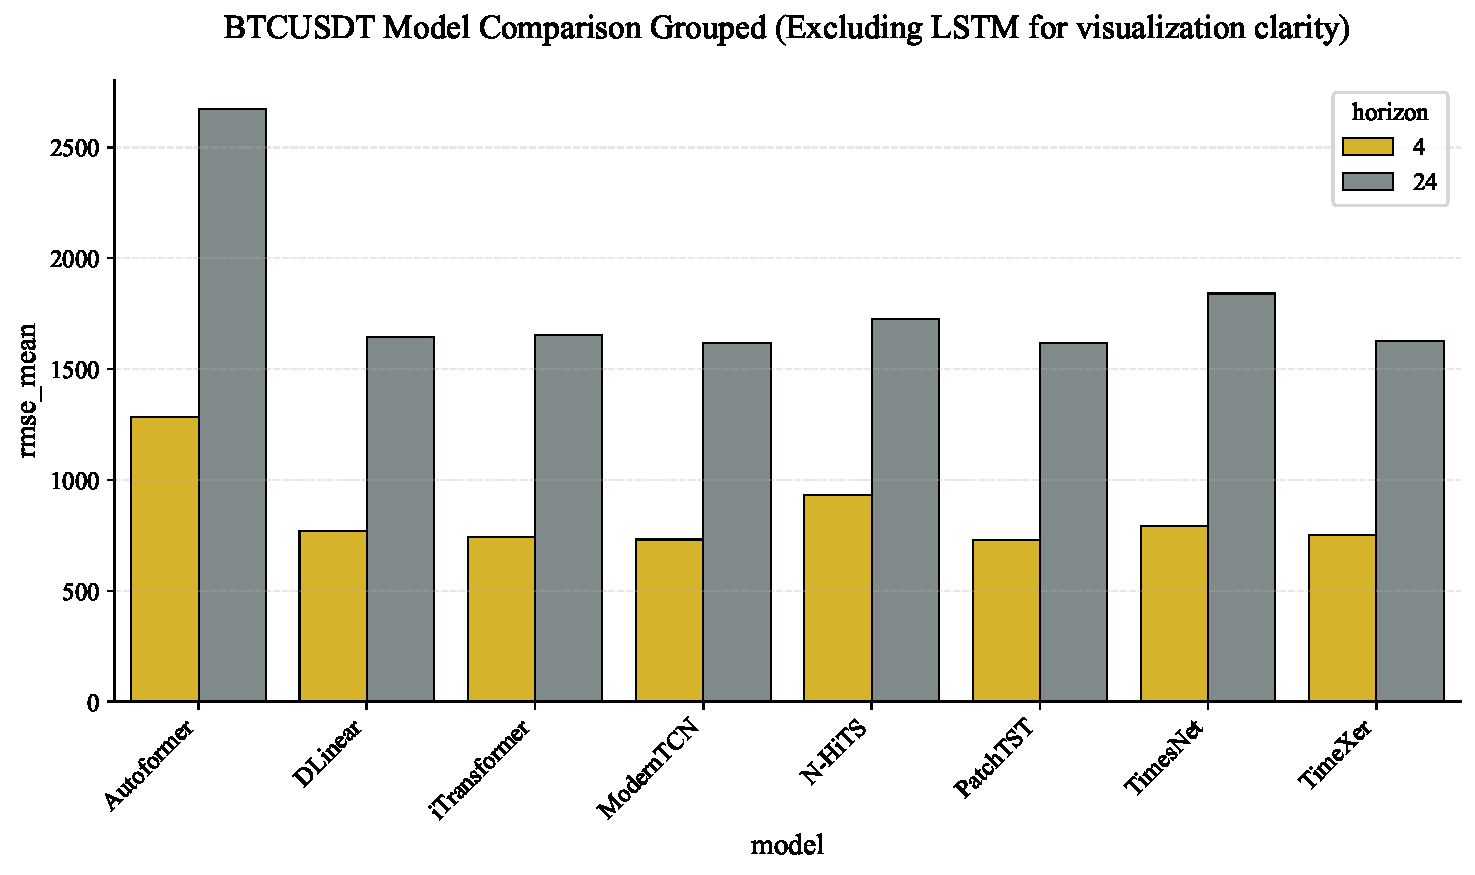
\includegraphics[width=\textwidth]{figures/04_category_analysis/asset_model_comparison_grouped_no_lstm.pdf}
  \caption{Cross-horizon \rmse comparison for eight modern architectures across twelve assets.  Each asset group displays \rmse at $\hfour$ and $\htwentyfour$.  The top-tier architectures (\moderntcn, \patchtst) maintain superior rankings across both horizons, while middle-tier models exhibit varying sensitivity to the forecast window length.}
  \label{fig:asset_model_comparison_grouped}
\end{figure}

\begin{figure}[htbp]
  \centering
  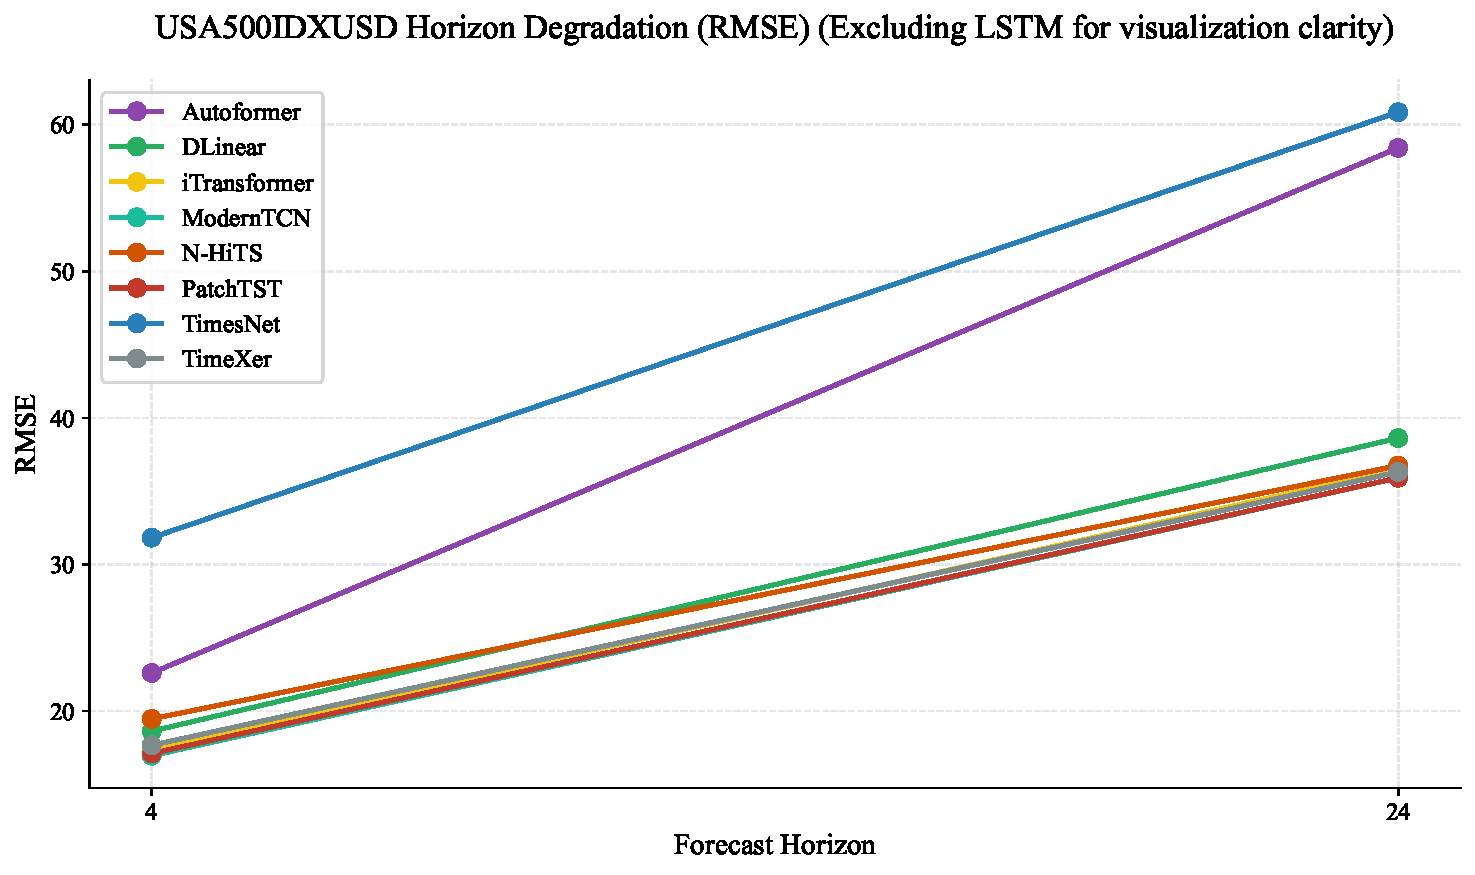
\includegraphics[width=0.75\textwidth]{figures/05_horizon_analysis/horizon_degradation_lineplot_no_lstm.pdf}
  \caption{Cross-horizon \rmse degradation for eight modern architectures across representative assets.  Lines connect each model's \rmse at $\hfour$ and $\htwentyfour$.  All architectures exhibit absolute error growth, but degradation magnitudes are architecture-dependent: \nhits degrades least, while \timesnet and \autoformer exhibit the steepest increase.  \moderntcn and \patchtst maintain top-tier performance at both horizons.  The full nine-model variant is provided in Appendix~\ref{sec:app_dual_plots}.}
  \label{fig:horizon_degradation}
\end{figure}


% --------------------------------------------------------------------------
\subsection{Seed Robustness and Variance Decomposition}
\label{sec:seed_robustness}

The two-factor variance decomposition (Table~\ref{tab:variance_decomposition}) is reported in three panels: raw \rmse, z-score normalised \rmse across all nine models, and z-score normalised \rmse excluding the \lstm outlier.

% =============================================================================
% Table 9 (revised): Two-Factor Variance Decomposition — z-normalised, dual panel
% =============================================================================
\begin{table}[htbp]
  \centering
  \begin{threeparttable}
  \caption{Two-factor variance decomposition of forecast \rmse.
    Raw (untransformed) and z-normalised (within each asset--horizon slot)
    panels are shown with and without \lstm.  Seed variance is negligible
    ($<\!0.1\,\%$) in all cases.}
  \label{tab:variance_decomposition}
  \setlength{\tabcolsep}{9pt}%
  \begin{tabular}{%
    l%
    S[table-format=2.2]%   Raw (all)
    S[table-format=2.2]%   z-norm all
    S[table-format=2.2]%   z-norm no LSTM
  }
    \toprule
    \textbf{Factor}
      & {\textbf{Raw (\%)}}
      & {\textbf{$z$-norm, all (\%)}}
      & {\textbf{$z$-norm, no \lstm (\%)}} \\
    \midrule
    \textbf{Model (architecture)}  & \bfseries 99.90 & \bfseries 48.32 & \bfseries 68.33 \\
    Seed (initialisation)          &  0.01 &  0.04 &  0.02 \\
    Residual (model$\times$slot)   &  0.09 & 51.64 & 31.66 \\
    \bottomrule
  \end{tabular}
  \begin{tablenotes}[flushleft]\footnotesize
    \item \textbf{Raw} panel: pooled variance decomposition on untransformed \rmse;
      \lstm's errors ($7\times$--$33\times$ higher than best model) dominate
      the model sum of squares, inflating the Model fraction to 99.90\,\%.
    \item \textbf{$z$-norm} panels: \rmse standardised within each
      (asset, horizon) slot before ANOVA, removing price-magnitude scale
      effects across asset classes.
    \item Residual ($\approx\!32$--$52\,\%$) reflects model$\times$slot
      interaction: each architecture has a context-dependent advantage on
      different asset--horizon combinations.  Seed variance ($<\!0.1\,\%$)
      is negligible across all three panels, validating the three-seed protocol.
  \end{tablenotes}
  \end{threeparttable}
\end{table}


\paragraph{Raw panel.}
On the original price scale, architecture absorbs 99.90\% of total sum-of-squares variance, versus 0.01\% for seed and 0.09\% for the residual.  This extreme dominance is largely an artefact of \lstm's outlier \rmse values: a single model $7{-}33\times$ above the median inflates $\mathrm{SS}_{\text{model}}$ relative to all other terms.

\paragraph{Z-normalised panels: all models.}
After z-scoring each model's \rmse within each (asset, horizon) slot, the architecture factor falls to \textbf{48.32\%}, seed to \textbf{0.04\%}, and the residual rises to \textbf{51.64\%}.  The large residual reflects genuine heterogeneity in which model excels on a given asset--horizon combination---a meaningful signal rather than noise.

\paragraph{Z-normalised panel: modern models only.}
Excluding \lstm, architecture recovers to \textbf{68.33\%} (seed: 0.02\%; residual: 31.66\%), confirming that architecture remains the dominant factor even among competitive modern models, though asset--horizon context contributes substantially.

In all three panels, seed variance is negligible ($\leq 0.04\%$): rankings are stable with respect to random initialisation and three seeds suffice.

Per-asset variance decompositions corroborate the global result.  At $\hfour$, architecture accounts for 99.75\% of variance on BTC/USDT, 97.44\% on EUR/USD, and 99.08\% on Dow Jones; seed fractions are 0.02\%, 0.35\%, and 0.01\% respectively.  Even EUR/USD, with the highest relative seed contribution, shows seed variance two orders of magnitude below the architecture factor.  At $\htwentyfour$, the pattern tightens further: architecture explains 99.86\% on BTC/USDT (seed: 0.02\%), confirming that initialisation effects diminish---rather than amplify---at longer horizons.

Figure~\ref{fig:robustness}(a) displays seed-to-seed \rmse variation per model as a violin plot.  Inter-seed variance is negligible relative to inter-model differences across all nine architectures: even \lstm, which has the highest absolute seed variance, shows seed-induced variation that is small relative to its distance from the nearest competitor.  Figure~\ref{fig:robustness}(b) provides a pie chart of the raw variance decomposition; the z-normalised breakdown appears in Table~\ref{tab:variance_decomposition}.  Per-asset seed-variance box plots and scatter plots for all three representative assets appear in Appendix~\ref{sec:app_robustness} (Figures~\ref{fig:app_seed_boxplot_h4}--\ref{fig:app_scatter_seed_h24}).

\begin{figure}[htbp]
  \centering
  \begin{subfigure}[b]{0.48\textwidth}
    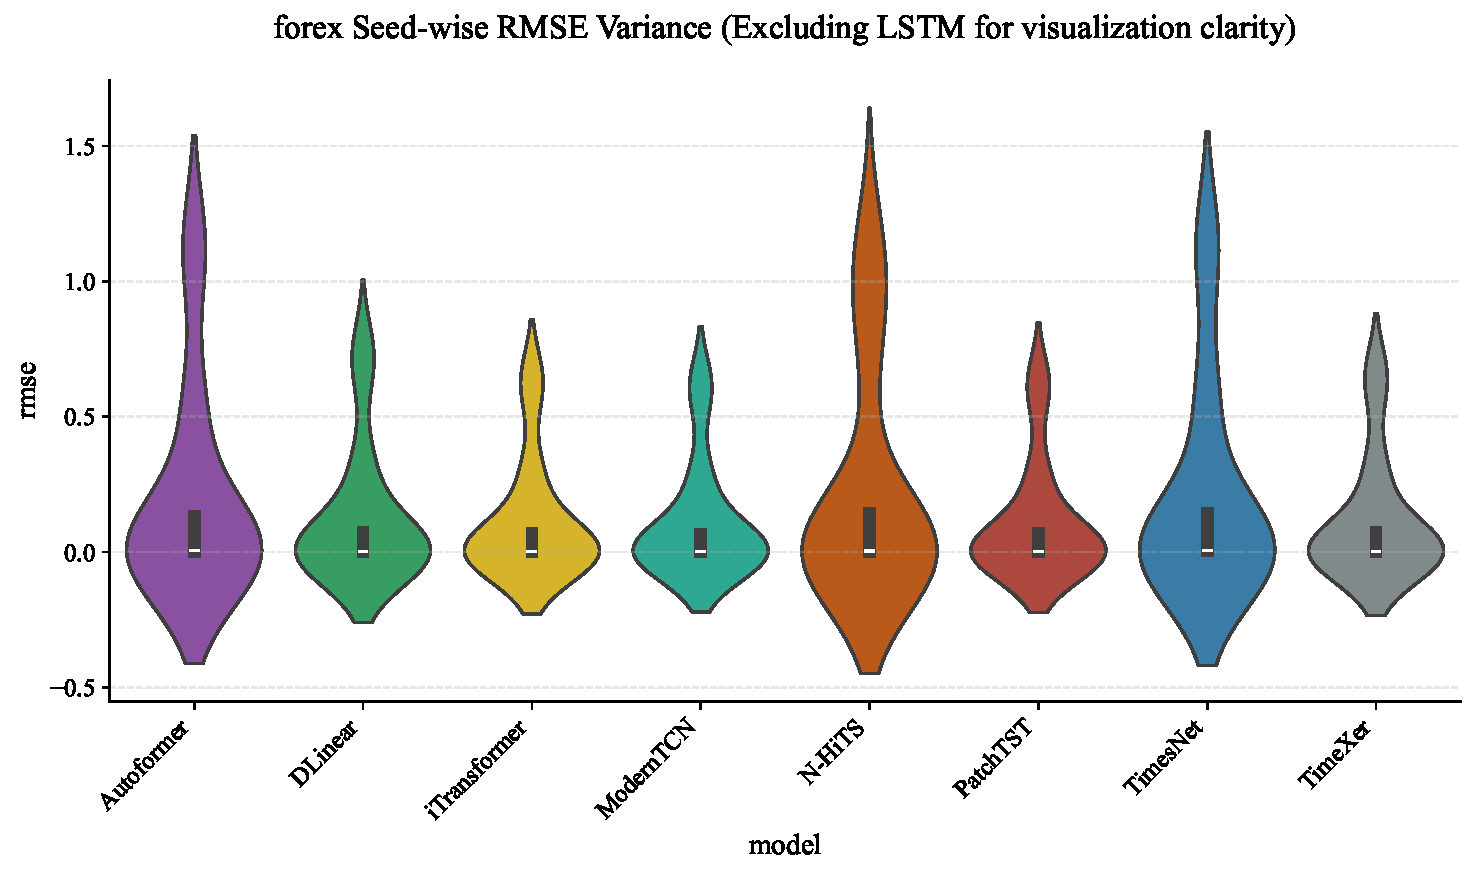
\includegraphics[width=\textwidth]{figures/06_robustness/seed_variance_violin.pdf}
    \caption{Seed variance violin plot.}
    \label{fig:seed_violin}
  \end{subfigure}
  \hfill
  \begin{subfigure}[b]{0.48\textwidth}
    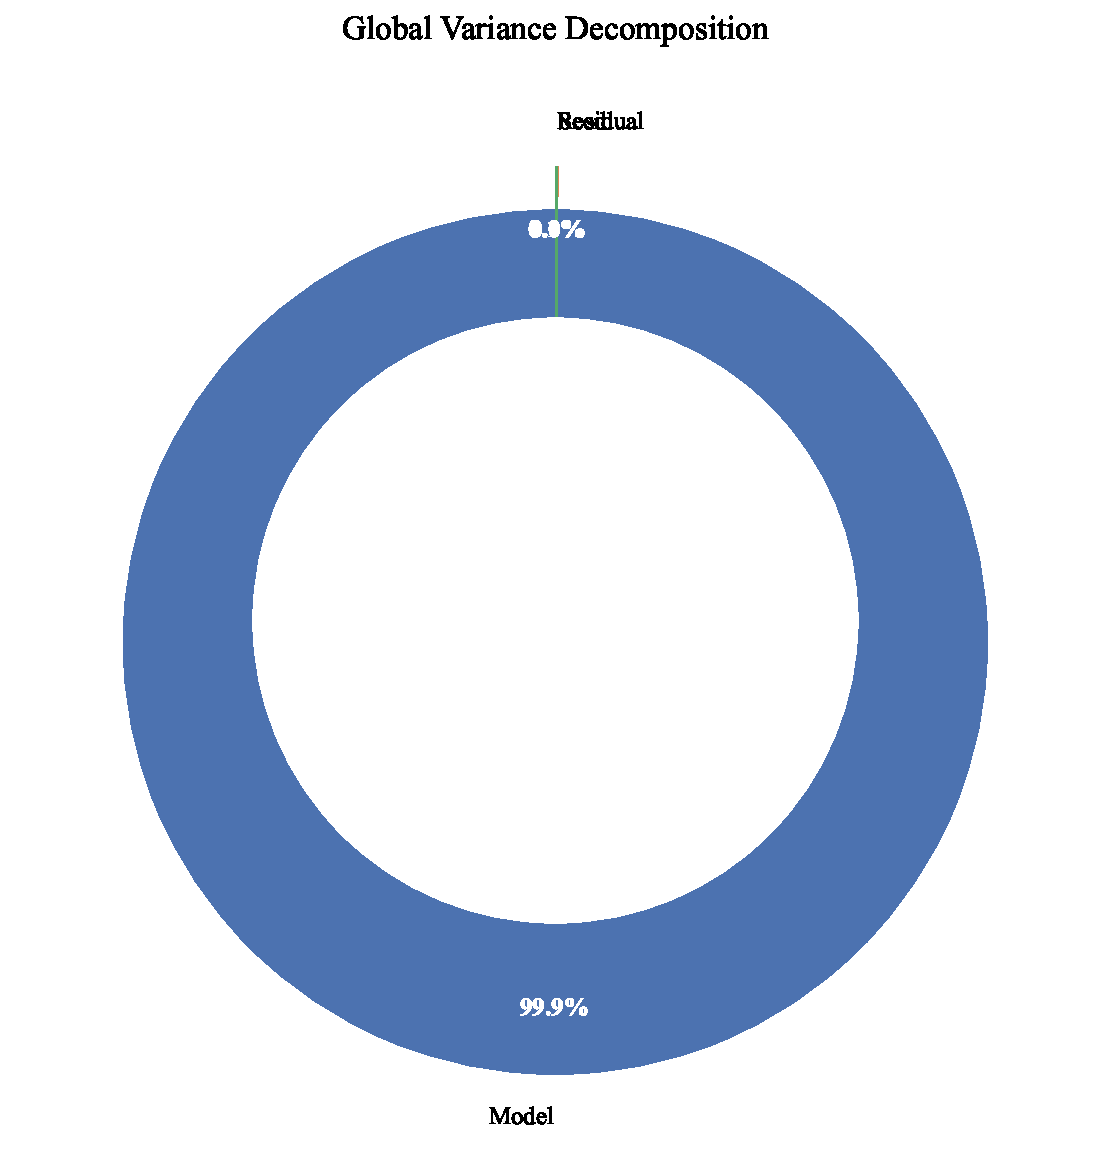
\includegraphics[width=\textwidth]{figures/06_robustness/variance_decomposition_pie.pdf}
    \caption{Variance decomposition (raw).}
    \label{fig:variance_pie}
  \end{subfigure}
  \caption{Seed robustness analysis.  (a)~Violin plot of seed-to-seed \rmse variation.  Inter-seed variation is negligible relative to inter-model differences across all nine architectures.  (b)~Two-factor variance decomposition on raw price-scale \rmse: architecture explains 99.90\%, seed 0.01\%, residual 0.09\%.  After z-score normalisation within each (asset, horizon) slot, the architecture share falls to 48.3\% (68.3\% excluding \lstm); see Table~\ref{tab:variance_decomposition} for the full dual-panel breakdown.}
  \label{fig:robustness}
\end{figure}


% --------------------------------------------------------------------------
\subsection{Directional Accuracy}
\label{sec:directional_accuracy}

Directional accuracy (\da) quantifies the fraction of forecasts that correctly predict the sign of the next price change.  Table~\ref{tab:directional_accuracy} reports mean \da\ per model, category, and horizon.


% siunitx setup
\sisetup{
  round-mode              = places,
  round-precision         = 2,
  detect-weight           = true,
  text-series-to-math     = true,
  table-number-alignment  = center
}

% =============================================================================
% Table 11: Directional Accuracy (per model, category, horizon)
% =============================================================================
\begin{table}[htbp]
  \centering
  \begin{threeparttable}
  \caption{Mean directional accuracy (\da, \%) per model, asset class, and
    horizon, averaged across assets within each category and over three
    seeds. Values close to 50\% indicate no systematic directional bias.}
  \label{tab:directional_accuracy}
  \footnotesize
  \setlength{\tabcolsep}{6pt}

  \begin{tabular}{
    l
    S[table-format=2.2]
    S[table-format=2.2]
    S[table-format=2.2]
    S[table-format=2.2]
    S[table-format=2.2]
    S[table-format=2.2]
  }
    \toprule
    & \multicolumn{2}{c}{\textbf{Crypto}}
    & \multicolumn{2}{c}{\textbf{Forex}}
    & \multicolumn{2}{c}{\textbf{Indices}} \\
    \cmidrule(lr){2-3}\cmidrule(lr){4-5}\cmidrule(lr){6-7}
    \textbf{Model}
      & {$h{=}4$} & {$h{=}24$}
      & {$h{=}4$} & {$h{=}24$}
      & {$h{=}4$} & {$h{=}24$} \\
    \midrule
    \autoformer     & 50.41 & 49.96 & 50.06 & 50.11 & 50.01 & 49.98 \\
    \dlinear        & 49.70 & 49.94 & 50.13 & 50.12 & 49.97 & 49.96 \\
    \itransformer   & 49.58 & 50.22 & 50.04 & 49.99 & 49.90 & 50.18 \\
    \lstm           & 49.73 & 50.07 & 50.08 & 49.95 & 49.88 & 49.95 \\
    \moderntcn      & 50.04 & 49.96 & 49.96 & 50.03 & 50.34 & 50.03 \\
    \nhits          & 50.05 & 49.87 & 50.02 & 50.03 & 50.78 & 49.92 \\
    \patchtst       & 50.07 & 49.85 & 50.10 & 49.98 & 50.42 & 49.95 \\
    \timesnet       & 50.57 & 50.34 & 50.05 & 49.88 & 50.27 & 50.18 \\
    \timexer        & 49.86 & 49.94 & 49.98 & 50.08 & 50.92 & 50.20 \\
    \bottomrule
  \end{tabular}

  \begin{tablenotes}[flushleft]\footnotesize
    \item Mean \da\ across all 54 model--category--horizon combinations is
      50.08\%, indistinguishable from a fair-coin baseline. No combination
      deviates meaningfully from 50\%. Values below 50\,\% indicate slight
      down-trend bias arising from scaling artefacts, not genuine negative
      directional skill.
  \end{tablenotes}

  \end{threeparttable}
\end{table}

Across all 9~models $\times$ 3~categories $\times$ 2~horizons ($=54$ combinations), mean \da\ is \textbf{50.08\%}.  No combination deviates meaningfully from 50\% and no horizon trend is discernible.

MSE-trained deep learning architectures produce directional forecasts equivalent to a fair coin flip on hourly financial data.  This is consistent with the weak-form efficient-market hypothesis at hourly resolution and with MSE training's regression-to-the-mean bias.  Section~\ref{sec:economic_interpretation} discusses implications for trading strategies.


% --------------------------------------------------------------------------
\subsection{Statistical Significance Tests}
\label{sec:statistical_tests}

Tables~\ref{tab:stat_tests_friedman}--\ref{tab:stat_tests_jt} report the full battery of statistical tests, providing formal confirmation of the descriptive findings in Sections~\ref{sec:global_rankings}--\ref{sec:directional_accuracy}.

% =============================================================================
% Table 10: Statistical Significance Tests — Comprehensive Summary
% Four panels: (A) Omnibus Friedman tests, (B) Cross-horizon Spearman + Stouffer,
%              (C) ICC seed reliability, (D) Jonckheere-Terpstra complexity test
% =============================================================================

% ---- Panel A: Omnibus Non-Parametric Tests ----------------------------------
\begin{table}[htbp]
  \centering
  \begin{threeparttable}
  \caption{Statistical significance tests — Panel~A: Friedman-Iman-Davenport
    omnibus tests.  \chisq: Friedman $\chi^2$ statistic (8~df); $F$:
    Iman-Davenport $F$-statistic; $n$: number of blocks (evaluation points).
    All tests reject \Hzero at $\alpha = 0.001$.}
  \label{tab:stat_tests_friedman}
  \setlength{\tabcolsep}{7pt}%
  \begin{tabular}{%
    l%              Scope
    S[table-format=3.2]%  chi^2
    S[table-format=3.2]%  F
    l%              df
    l%              p-value
    c%              n
  }
    \toprule
    \textbf{Scope}
      & {\chisq(8)}
      & {$F$}
      & {df}
      & {$p$}
      & {$n$} \\
    \midrule
    Global (all 12 assets, $h\in\{4,24\}$) & 156.49 & 101.36 & (8,\;184) & $<\!10^{-15}$ & 24 \\
    Crypto (4~assets, $h\in\{4,24\}$)      &  49.23 &  23.34 & (8,\;56)  & $<\!10^{-15}$ &  8 \\
    Forex (4~assets, $h\in\{4,24\}$)       &  56.00 &  49.00 & (8,\;56)  & $<\!10^{-15}$ &  8 \\
    Indices (4~assets, $h\in\{4,24\}$)     &  60.40 & 117.44 & (8,\;56)  & $<\!10^{-15}$ &  8 \\
    \bottomrule
  \end{tabular}
  \end{threeparttable}
\end{table}

% ---- Panel B: Cross-Horizon Spearman + Stouffer ----------------------------
\begin{table}[htbp]
  \centering
  \begin{threeparttable}
  \caption{Statistical significance tests — Panel~B: Spearman rank
    correlations between model rankings at $\hfour$ and $\htwentyfour$, plus
    Stouffer combined test.  Rankings are based on mean \rmse across three
    seeds for each of the nine architectures ($n = 9$ per asset).
    All 12 per-asset correlations are significant at $\alpha = 0.05$.}
  \label{tab:stat_tests_spearman}
  \setlength{\tabcolsep}{8pt}%
  \begin{tabular}{%
    l%         Category
    l%         Asset
    S[table-format=1.4]%  rho
    l%         p-value
  }
    \toprule
    \textbf{Category} & \textbf{Asset}
      & {Spearman $\rho$}
      & {$p$-value} \\
    \midrule
    Crypto  & ADA/USDT          & 0.683 & 0.0424 \\
    Crypto  & BNB/USDT          & 0.917 & 0.0005 \\
    Crypto  & BTC/USDT          & 0.917 & 0.0005 \\
    Crypto  & ETH/USDT          & 0.783 & 0.0125 \\
    \addlinespace
    Forex   & AUD/USD           & 0.867 & 0.0025 \\
    Forex   & EUR/USD           & 1.000 & $<\!10^{-9}$ \\
    Forex   & GBP/USD           & 0.800 & 0.0096 \\
    Forex   & USD/JPY           & 0.950 & 0.0001 \\
    \addlinespace
    Indices & DAX               & 0.883 & 0.0016 \\
    Indices & Dow Jones         & 0.867 & 0.0025 \\
    Indices & S\&P~500          & 0.967 & $<\!10^{-4}$ \\
    Indices & NASDAQ~100        & 0.983 & $<\!10^{-5}$ \\
    \midrule
    \multicolumn{2}{l}{\textbf{Stouffer combined} ($n = 12$ assets)}
      & \multicolumn{1}{S[table-format=1.2]}{6.17}
      & $3.47\times10^{-10}$ \\
    \bottomrule
  \end{tabular}
  \begin{tablenotes}[flushleft]\footnotesize
    \item Stouffer combined $Z$-statistic aggregates the 12 per-asset
      one-sided Spearman $p$-values using the inverse-normal method.
      The global $p = 3.47\times10^{-10}$ confirms that cross-horizon
      rank stability is a systematic property of the benchmark.
  \end{tablenotes}
  \end{threeparttable}
\end{table}

% ---- Panel C: ICC Seed Reliability ------------------------------------------
\begin{table}[htbp]
  \centering
  \begin{threeparttable}
  \caption{Statistical significance tests — Panel~C: Intraclass Correlation
    Coefficient (\icc; two-way mixed, absolute agreement) for three
    representative assets at $\htwentyfour$.  High \icc values confirm
    negligible seed-to-seed variation relative to inter-model differences.}
  \label{tab:stat_tests_icc}
  \setlength{\tabcolsep}{8pt}%
  \begin{tabular}{%
    l%         Asset
    S[table-format=1.4]%  ICC
    S[table-format=4.1]%  F
    l%         p-value
  }
    \toprule
    \textbf{Asset ($h{=}24$)}
      & {\icc}
      & {$F$-statistic}
      & {$p$-value} \\
    \midrule
    BTC/USDT     & 0.9982 & 1650.2 & $<\!10^{-15}$ \\
    EUR/USD      & 0.9904 &  309.6 & $<\!10^{-15}$ \\
    S\&P~500     & 0.9987 & 2255.6 & $<\!10^{-15}$ \\
    \bottomrule
  \end{tabular}
  \begin{tablenotes}[flushleft]\footnotesize
    \item Each \icc computed over 9 models $\times$ 3 seeds.  $F$-statistic
      tests \Hzero: all seed means are equal.  Values above 0.99 indicate
      that $>99\%$ of inter-model variance is attributable to architecture
      rather than random initialisation.
  \end{tablenotes}
  \end{threeparttable}
\end{table}

% ---- Panel D: Jonckheere-Terpstra Complexity Monotonicity Test --------------
\begin{table}[htbp]
  \centering
  \begin{threeparttable}
  \caption{Statistical significance tests — Panel~D:
    Jonckheere-Terpstra (\jt) test for a monotonic relationship between
    model complexity (parameter count) and \rmse rank.  A significant
    positive result would indicate that more parameters reliably yield
    better ranks.  Three complexity groups: $\leq\!30\mathrm{K}$,
    $30\mathrm{K}$--$200\mathrm{K}$, $>\!200\mathrm{K}$ parameters.}
  \label{tab:stat_tests_jt}
  \setlength{\tabcolsep}{8pt}%
  \begin{tabular}{%
    l%         Category
    c%         Horizon
    S[table-format=+1.4]%  JT z-stat
    S[table-format=1.4]%   p-value
    c%         Conclusion
  }
    \toprule
    \textbf{Category}
      & \textbf{Horizon}
      & {\jt $z$}
      & {$p$-value}
      & \textbf{Monotonic?} \\
    \midrule
    Crypto  & 4  & +0.348 & 0.364 & No \\
    Crypto  & 24 & -0.348 & 0.636 & No \\
    \addlinespace
    Forex   & 4  & +0.377 & 0.353 & No \\
    Forex   & 24 & -0.290 & 0.614 & No \\
    \addlinespace
    Indices & 4  & -1.248 & 0.894 & No \\
    Indices & 24 & -1.480 & 0.931 & No \\
    \bottomrule
  \end{tabular}
  \begin{tablenotes}[flushleft]\footnotesize
    \item No test achieves significance ($\alpha = 0.05$); all $p > 0.35$.
      Negative $z$ values indicate a tendency for \emph{fewer} parameters
      to yield better ranks, consistent with the Pareto frontier defined
      by \dlinear, \patchtst, and \moderntcn (Figure~\ref{fig:complexity}).
  \end{tablenotes}
  \end{threeparttable}
\end{table}


\paragraph{Global Friedman-Iman-Davenport test.}
The Friedman-Iman-Davenport test on all 24~evaluation points (12~assets $\times$ 2~horizons) yields $F(8,184) = 101.36$, $p < 10^{-15}$ (Friedman $\chisq(8) = 156.49$, $p = 8.67 \times 10^{-30}$), firmly rejecting the null hypothesis that all nine architectures perform equivalently.  Table~\ref{tab:stat_tests_friedman} indicates that exactly the same conclusion holds within every individual asset class: crypto ($F = 23.34$), forex ($F = 49.00$), and indices ($F = 117.44$), each with $p < 10^{-15}$.

\paragraph{Post-hoc Holm-Wilcoxon pairwise tests (global).}
Of the $\binom{9}{2} = 36$ pairwise Wilcoxon comparisons at the global level ($n = 24$ observations), 33~are statistically significant after Holm correction ($\alpha = 0.05$).  The three non-significant pairs are all \emph{intra-tier}: \timexer~vs.~\itransformer ($p_\text{Holm} = 0.480$), \autoformer~vs.~\timesnet ($p_\text{Holm} = 0.529$), and \dlinear~vs.~\nhits ($p_\text{Holm} = 0.529$) --- confirming that only neighbouring models within the same performance tier are statistically indistinguishable.

At the per-category level ($n = 8$: 4~assets $\times$ 2~horizons), no pairwise comparison reaches significance after Holm correction (all $p_\text{Holm} > 0.28$).  This reflects a \emph{power constraint}, not an absence of effect: with $n = 8$, the minimum achievable Wilcoxon $p$-value is $0.0078$; the Holm step-down procedure requires the most extreme raw $p$-value to beat $0.05/36 = 0.0014$, which is unattainable at this sample size.  The per-category result is thus consistent with---and subsumed by---the decisive global test.

\paragraph{Critical difference diagram.}
Figure~\ref{fig:cd_diagram} visualises the Holm-Wilcoxon significance structure as a critical difference (CD) diagram.  The horizontal axis represents mean rank across all $N = 24$ evaluation blocks ($k = 9$ models); lower values denote superior performance.  Each model is placed at its exact mean rank derived from \texttt{global\_ranking\_aggregated.csv}.  Thick horizontal bars connect pairs that are \emph{not} statistically distinguishable after Holm correction ($\alpha = 0.05$); all unlabelled pairs are significant.

Three intra-tier equivalence groups emerge directly from the pairwise test results.  Within the middle tier, \itransformer (rank~3.667) and \timexer (rank~4.292) are statistically indistinguishable ($p_\text{Holm} = 0.480$), as are \dlinear (rank~4.958) and \nhits (rank~5.250) ($p_\text{Holm} = 0.529$).  Within the bottom tier, \timesnet (rank~7.708) and \autoformer (rank~7.833) are statistically equivalent ($p_\text{Holm} = 0.529$).  All 33~remaining comparisons are statistically significant, including every cross-tier comparison.  In particular, the top-tier boundary is unambiguous: \moderntcn (rank~1.333) and \patchtst (rank~2.000) are each significantly superior to every model in the middle and bottom tiers ($p_\text{Holm} \leq 0.028$ in all cases).

The bracketed interval labelled $\cdfive = 2.451$ in the upper-left corner displays the Nemenyi critical difference computed as $\mathrm{CD} = q_{0.05}(9)\sqrt{k(k+1)/(6N)} = 3.102 \times \sqrt{90/144}$, where $q_{0.05}(9) = 3.102$ is the studentised range critical value at $\alpha = 0.05$ for $k = 9$ and $N = 24$.  This bracket is shown as a reference only; all significance claims in this paper are derived from the more powerful Holm-corrected Wilcoxon procedure rather than the Nemenyi threshold.  Notably, the full rank span from \moderntcn to \lstm ($\Delta r = 6.625$) exceeds $2.7 \times \cdfive$, confirming that the top-to-bottom separation is not a boundary case but an overwhelming statistical gap.

\begin{figure}[htbp]
  \centering
  % Critical Difference (CD) Diagram
% k = 9 models, N = 24 evaluation blocks (12 assets x 2 forecast horizons)
% Primary source: results/benchmark/global_summary/tables/global_ranking_aggregated.csv
% Post-hoc test: Holm--Wilcoxon (alpha = 0.05)
% Non-significant pairs (holm_wilcoxon.csv, significant=False):
%   iTransformer -- TimeXer   (p_holm = 0.4800)
%   DLinear      -- N-HiTS    (p_holm = 0.5287)
%   TimesNet     -- Autoformer (p_holm = 0.5287)
% Nemenyi CD = q_{0.05}(9) * sqrt(k(k+1)/(6N))
%            = 3.102 * sqrt(90/144) = 2.4507  [reference bracket only]
%
% x-coordinate mapping:  x(r) = (r - 1) * 1.5  cm
%   ModernTCN    rank 1.3333  ->  x = 0.5000
%   PatchTST     rank 2.0000  ->  x = 1.5000
%   iTransformer rank 3.6667  ->  x = 4.0000
%   TimeXer      rank 4.2917  ->  x = 4.9375
%   DLinear      rank 4.9583  ->  x = 5.9375
%   N-HiTS       rank 5.2500  ->  x = 6.3750
%   TimesNet     rank 7.7083  ->  x = 10.0625
%   Autoformer   rank 7.8333  ->  x = 10.2500
%   LSTM         rank 7.9583  ->  x = 10.4375
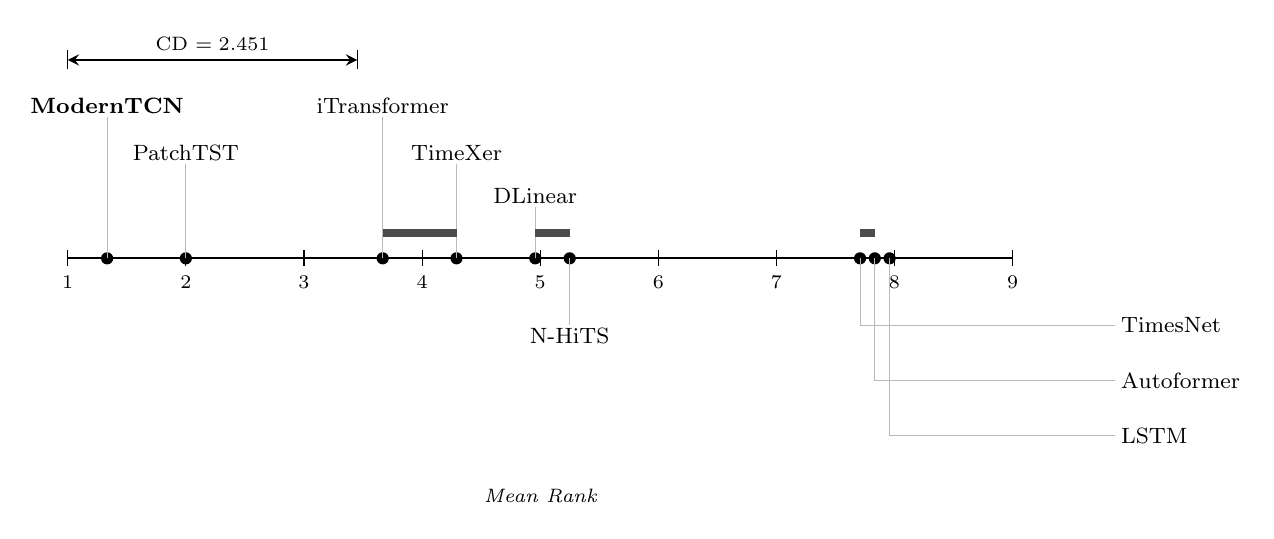
\begin{tikzpicture}[font=\small]

% =====================================================================
% Horizontal rank axis  (rank 1 = left/best, rank 9 = right/worst)
% =====================================================================
\draw[thick] (0,0) -- (12,0);

% Integer rank tick marks and labels
\foreach \r in {1,...,9}{
  \pgfmathsetmacro{\xt}{(\r-1)*1.5}
  \draw (\xt, 0.10) -- (\xt,-0.10);
  \node[below, font=\scriptsize] at (\xt,-0.10) {\r};
}

% =====================================================================
% Model dot markers at exact mean-rank positions
% =====================================================================
\foreach \xm in {0.5000, 1.5000, 4.0000, 4.9375, 5.9375,
                 6.3750, 10.0625, 10.2500, 10.4375}{
  \fill[black] (\xm,0) circle[radius=2.2pt];
}

% =====================================================================
% Top-half models: vertical stems + labels ABOVE axis
% Heights alternated to prevent label overlap
% =====================================================================

% ModernTCN   rank=1.3333   x=0.5000   h=1.8
\draw[gray!55,thin] (0.5000,0) -- (0.5000,1.8);
\node[above, inner sep=1pt, font=\footnotesize\bfseries]
  at (0.5000,1.8) {ModernTCN};

% PatchTST    rank=2.0000   x=1.5000   h=1.2
\draw[gray!55,thin] (1.5000,0) -- (1.5000,1.2);
\node[above, inner sep=1pt, font=\footnotesize]
  at (1.5000,1.2) {PatchTST};

% iTransformer   rank=3.6667   x=4.0000   h=1.8
\draw[gray!55,thin] (4.0000,0) -- (4.0000,1.8);
\node[above, inner sep=1pt, font=\footnotesize]
  at (4.0000,1.8) {iTransformer};

% TimeXer   rank=4.2917   x=4.9375   h=1.2
\draw[gray!55,thin] (4.9375,0) -- (4.9375,1.2);
\node[above, inner sep=1pt, font=\footnotesize]
  at (4.9375,1.2) {TimeXer};

% DLinear   rank=4.9583   x=5.9375   h=0.65
\draw[gray!55,thin] (5.9375,0) -- (5.9375,0.65);
\node[above, inner sep=1pt, font=\footnotesize]
  at (5.9375,0.65) {DLinear};

% =====================================================================
% Bottom-half models: stems + labels BELOW axis
% =====================================================================

% N-HiTS   rank=5.2500   x=6.3750   depth=0.85
\draw[gray!55,thin] (6.3750,0) -- (6.3750,-0.85);
\node[below, inner sep=1pt, font=\footnotesize]
  at (6.3750,-0.85) {N-HiTS};

% TimesNet / Autoformer / LSTM are within 0.375 cm of each other.
% Use staggered depths + horizontal leaders to a right-margin label column.

% TimesNet   rank=7.7083   x=10.0625   depth=0.85 -> leader to x=13.3
\draw[gray!55,thin] (10.0625,0) -- (10.0625,-0.85) -- (13.3,-0.85);
\node[right, inner sep=2pt, font=\footnotesize] at (13.3,-0.85) {TimesNet};

% Autoformer   rank=7.8333   x=10.2500   depth=1.55 -> leader to x=13.3
\draw[gray!55,thin] (10.2500,0) -- (10.2500,-1.55) -- (13.3,-1.55);
\node[right, inner sep=2pt, font=\footnotesize] at (13.3,-1.55) {Autoformer};

% LSTM   rank=7.9583   x=10.4375   depth=2.25 -> leader to x=13.3
\draw[gray!55,thin] (10.4375,0) -- (10.4375,-2.25) -- (13.3,-2.25);
\node[right, inner sep=2pt, font=\footnotesize] at (13.3,-2.25) {LSTM};

% =====================================================================
% Significance clique bars (Holm--Wilcoxon, alpha=0.05)
% Thick bars at y=0.32 connecting models NOT significantly different.
% Three non-significant pairs from global holm_wilcoxon.csv.
% =====================================================================

% Clique 1: iTransformer (4.0000) -- TimeXer (4.9375)
\draw[line width=2.8pt, black!70] (4.0000,0.32) -- (4.9375,0.32);

% Clique 2: DLinear (5.9375) -- N-HiTS (6.3750)
\draw[line width=2.8pt, black!70] (5.9375,0.32) -- (6.3750,0.32);

% Clique 3: TimesNet (10.0625) -- Autoformer (10.2500)
\draw[line width=2.8pt, black!70] (10.0625,0.32) -- (10.2500,0.32);

% =====================================================================
% Nemenyi CD reference bracket (top-left)
% CD = 3.102 * sqrt(9*10/(6*24)) = 2.4507 rank units
% Axis span = 2.4507 * 1.5 = 3.6761 cm
% =====================================================================
\draw[thick,<->,>=stealth] (0,2.52) -- (3.6761,2.52);
\draw[thin] (0,2.40) -- (0,2.65);
\draw[thin] (3.6761,2.40) -- (3.6761,2.65);
\node[above, font=\scriptsize] at (1.8381,2.52) {CD $= 2.451$};

% =====================================================================
% Axis label
% =====================================================================
\node[below, font=\scriptsize\itshape] at (6.0,-2.80) {Mean Rank};

\end{tikzpicture}

  \caption{Critical difference diagram for \nmodels forecasting architectures
           across $N = 24$ evaluation blocks (12~assets $\times$ 2~horizons).
           Models are placed at their exact mean \rmse rank; lower rank is better.
           Thick horizontal bars connect models that are \emph{not} statistically
           distinguishable at $\alpha = 0.05$ under Holm-corrected Wilcoxon tests
           (\texttt{holm\_wilcoxon.csv}):
           \itransformer--\timexer ($p_\text{Holm} = 0.480$),
           \dlinear--\nhits ($p_\text{Holm} = 0.529$), and
           \timesnet--\autoformer ($p_\text{Holm} = 0.529$).
           All other 33 pairwise comparisons are significant.
           The bracketed interval (upper left) shows the Nemenyi critical
           difference $\cdfive = 2.451$ ($k = 9$, $N = 24$, $q_{0.05} = 3.102$)
           for reference only.}
  \label{fig:cd_diagram}
\end{figure}

\paragraph{Cross-horizon Spearman rank correlations and Stouffer combination.}
Table~\ref{tab:stat_tests_spearman} reports the Spearman $\rho$ between model rankings at $\hfour$ and $\htwentyfour$ for all twelve assets.  All 12~correlations are positive and statistically significant ($p < 0.05$), with $\rho$ ranging from $0.683$ (ADA/USDT) to $1.000$ (EUR/USD).  The Stouffer combined statistic $\stoufferz = 6.17$ ($p = 3.47 \times 10^{-10}$) confirms that cross-horizon rank stability is a globally systematic property: no single architecture's ranking collapses between the two horizons.

\paragraph{Intraclass Correlation Coefficient (\icc).}
\icc(3,k) analysis for three representative assets at $\htwentyfour$ (Table~\ref{tab:stat_tests_icc}) yields ICC $> 0.990$ in all cases, with $F$-statistics ranging from 309.6 to 2255.6 ($p < 10^{-15}$).  These values indicate that more than 99\% of inter-model variance arises from architecture rather than random initialisation, corroborating the $\leq 0.04\%$ seed contribution in Table~\ref{tab:variance_decomposition}.  At $\hfour$, ICC remains high: 0.9966 (BTC/USDT, $F = 873.9$), 0.9668 (EUR/USD, $F = 88.4$), and 0.9864 (Dow Jones, $F = 218.2$), all with $p < 10^{-11}$.  EUR/USD's comparatively lower $\hfour$ ICC reflects the tighter model clustering on this low-volatility pair rather than genuine seed instability, as even 96.7\% remains far above conventional reliability thresholds.

\paragraph{Diebold-Mariano pairwise tests.}
For BTC/USDT at $\htwentyfour$, Holm-corrected Diebold-Mariano (\dm) tests show that the top cluster (\moderntcn, \patchtst, \timexer, \dlinear, \itransformer) is internally partially distinguishable.  Specifically, \moderntcn~vs.~\patchtst is not significant ($p_\text{Holm} = 0.453$), and \moderntcn~vs.~\timexer is borderline ($p_\text{Holm} = 0.094$), while all comparisons to \lstm, \autoformer, and \timesnet are highly significant ($p < 10^{-14}$).

EUR/USD at $\htwentyfour$ exhibits a sharper separation structure.  \moderntcn is statistically \emph{distinguishable} from \patchtst ($t_\text{DM} = -10.17$, $p_\text{Holm} = 2.77 \times 10^{-24}$) and from \timexer ($t_\text{DM} = -9.21$, $p_\text{Holm} = 3.30 \times 10^{-20}$)---unlike BTC/USDT, where these top-tier differences are not significant.  The non-significant pairs on EUR/USD are \dlinear~vs.~\patchtst ($p_\text{Holm} = 0.122$), \dlinear~vs.~\timexer ($p_\text{Holm} = 0.187$), \dlinear~vs.~\itransformer ($p_\text{Holm} = 0.187$), and \itransformer~vs.~\patchtst ($p_\text{Holm} = 0.717$).  Thus, on the most liquid and low-noise forex pair, \moderntcn's superiority is statistically unambiguous, whereas the middle cluster (\dlinear, \itransformer, \patchtst, \timexer) remains internally indistinguishable.  This asset-dependent DM separability suggests that the statistical power to discriminate the top two architectures depends on the signal-to-noise properties of the underlying market.

These results confirm that the top-tier boundary (\moderntcn and \patchtst) is not artefactual, but that fine-grained rankings within the three-to-five-model cluster should be interpreted with appropriate caution across individual assets.

\paragraph{Jonckheere-Terpstra test for complexity monotonicity.}
The Jonckheere-Terpstra (\jt) test for a monotonic rank-descending trend with increasing parameter count finds no significant relationship in any of the six category--horizon combinations tested (all $p > 0.35$; Table~\ref{tab:stat_tests_jt}).  Four of the six $z$-values are negative, indicating that fewer parameters tend to yield \emph{better} ranks on average.  This formally corroborates the non-monotonic complexity--performance finding (Section~\ref{sec:complexity}).

\paragraph{Directional accuracy z-tests.}
One-sample z-tests on directional accuracy confirm that no architecture's \da\ deviates significantly from the 50\% null (all Holm-corrected $p > 0.43$ for BTC/USDT at $\htwentyfour$), corroborating the aggregate finding in Section~\ref{sec:directional_accuracy}.  The test with the largest $|z|$ is \itransformer ($z = 0.263$, $p_\text{Holm} = 1.0$), confirming that no model possesses directional skill at this resolution.


% --------------------------------------------------------------------------
\subsection{Complexity--Performance Relationship}
\label{sec:complexity}

The relationship between model complexity, measured by trainable parameter count, and forecasting performance is shown in Figure~\ref{fig:complexity}.  The analysis focuses on modern architectures, excluding the \lstm baseline.

\begin{figure}[htbp]
  \centering
  \begin{subfigure}[b]{0.48\textwidth}
    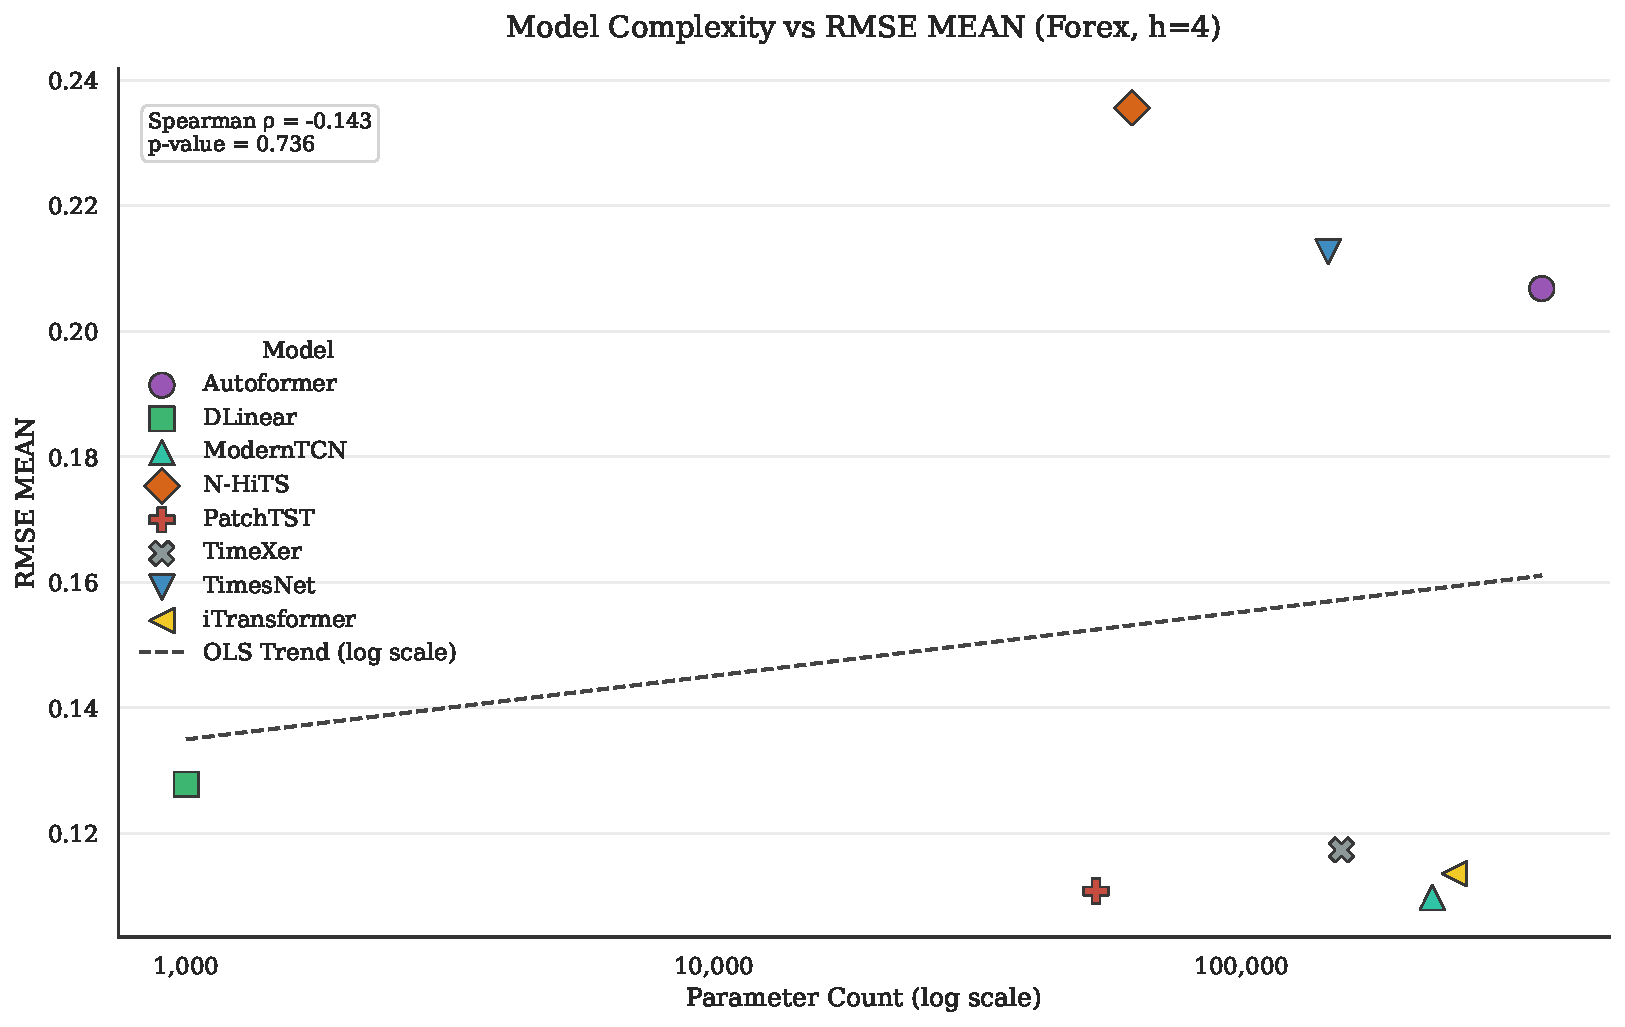
\includegraphics[width=\textwidth]{figures/07_efficiency/complexity_vs_performance_h4_no_lstm.pdf}
    \caption{Horizon $h=4$.}
    \label{fig:complexity_h4}
  \end{subfigure}
  \hfill
  \begin{subfigure}[b]{0.48\textwidth}
    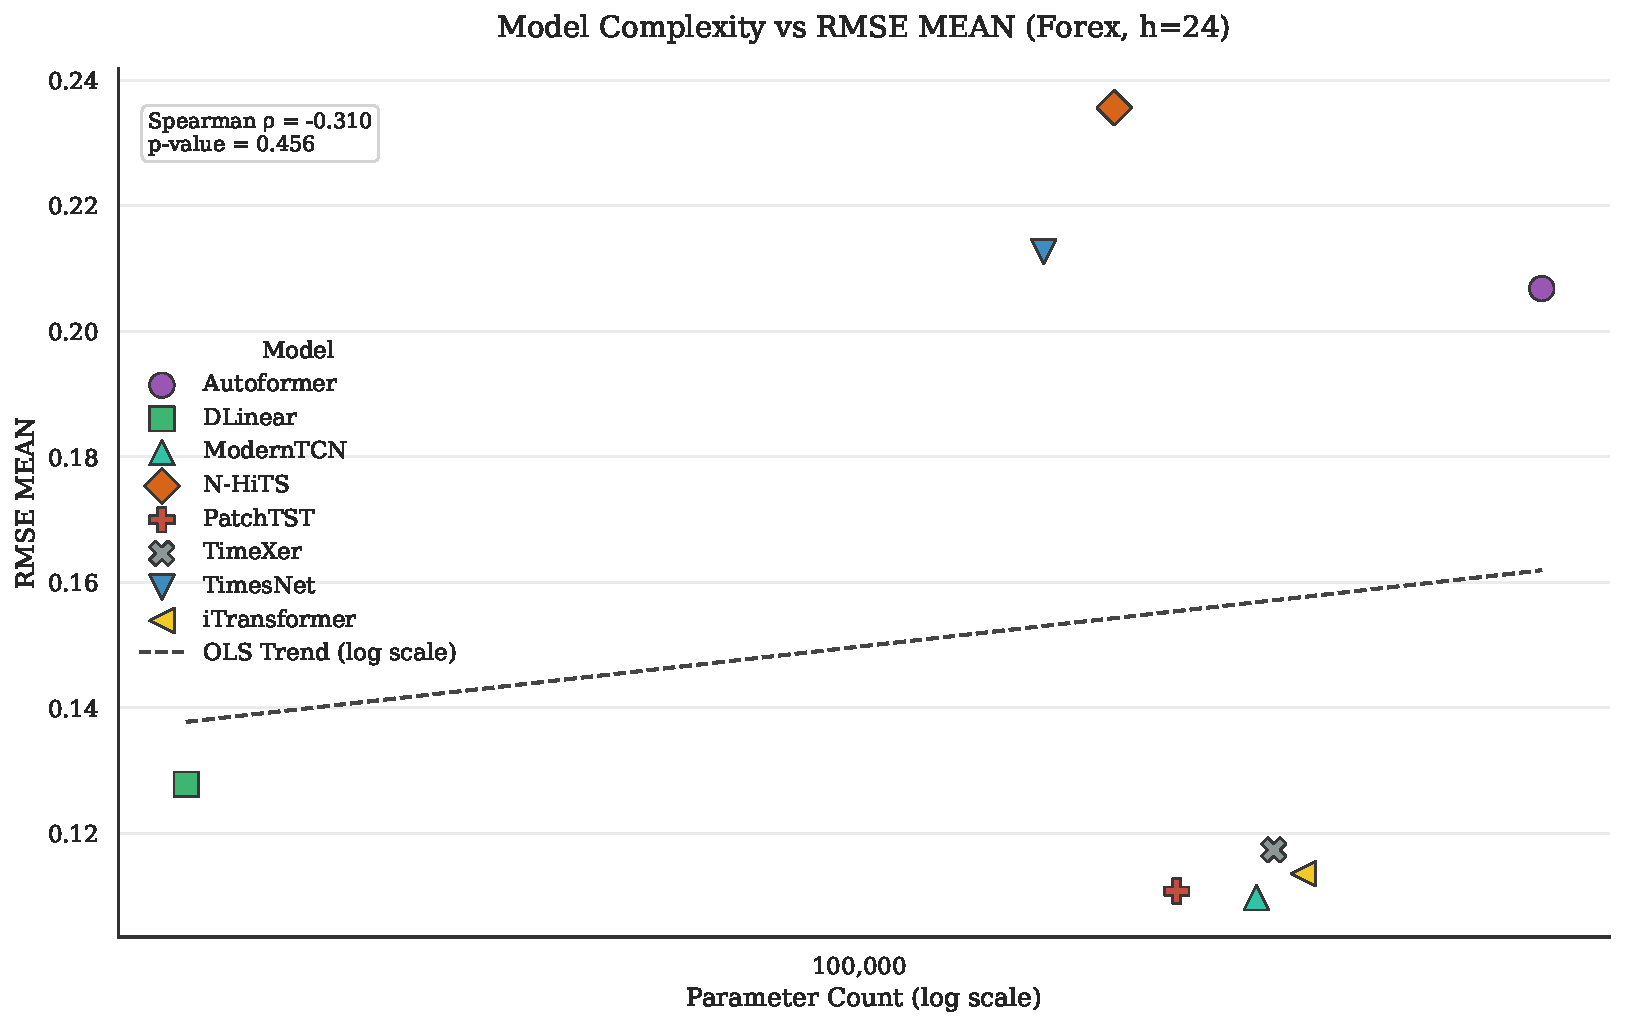
\includegraphics[width=\textwidth]{figures/07_efficiency/complexity_vs_performance_h24_no_lstm.pdf}
    \caption{Horizon $h=24$.}
    \label{fig:complexity_h24}
  \end{subfigure}
  \caption{Complexity--performance trade-off (excluding \lstm). The horizontal axis represents the number of trainable parameters (log scale); the vertical axis represents the mean \rmse rank across all assets and seeds. The Pareto frontier is clearly defined by \dlinear, \patchtst, and \moderntcn.}
  \label{fig:complexity}
\end{figure}

The empirical results reveal several insights:

\paragraph{Pareto-efficient architectures.}
A distinct Pareto frontier is defined by \dlinear, \patchtst, and \moderntcn.  \dlinear (approx.\ 1{,}000 parameters) represents the extreme efficiency point, achieving mid-tier performance (rank~5) with minimal capacity.  \patchtst (approx.\ 103K) and \moderntcn (approx.\ 230K) occupy the optimal region, providing the lowest \rmse ranks globally by deploying parameters into inductive biases suited to financial time series.

\paragraph{Diminishing returns at high complexity.}
Beyond approximately $2.5 \times 10^5$ parameters, returns diminish sharply.  \autoformer (approx.\ 438K) and \itransformer (approx.\ 253K) do not improve commensurately with their larger capacity. \autoformer's rank is consistently lower than the simpler \dlinear, suggesting that excess capacity without appropriate temporal decomposition may lead to overfitting on volatile OHLCV features.

\paragraph{Horizon consistency.}
Comparing Figure~\ref{fig:complexity_h4} and Figure~\ref{fig:complexity_h24} shows that the efficiency profile remains stable across horizons.  Absolute errors increase at $h=24$, but relative model positions on the complexity--performance plane are preserved, indicating that architectural efficiency is a robust property of the model design.

% --------------------------------------------------------------------------
\subsection{Qualitative Forecast Fidelity}
\label{sec:qualitative_fidelity}

Quantitative metrics efficiently rank architectures but compress multi-dimensional forecast behaviour into scalar summaries.  This subsection complements the tabular evidence with actual-versus-predicted overlays, organised along three dimensions: short-horizon tracking ($\hfour$), medium-horizon behaviour ($\htwentyfour$, step~12), and long-horizon degradation ($\htwentyfour$, step~24).  All plots use seed~123; analogous patterns hold across seeds given the near-zero seed variance established in Section~\ref{sec:seed_robustness}.

% - - - - - - - - - - - - - - - - - - - - - - - - - - - - - - - - - - - - -
\paragraph{Short-horizon tracking fidelity ($h = 4$, steps 1 and 4).}

Figure~\ref{fig:pred_btc_h4_step1_step4} presents \moderntcn's actual-versus-predicted overlay on BTC/USDT at $\hfour$ for steps~1 and~4 of the forecast vector.  At step~1 (Figure~\ref{fig:pred_btc_h4_step1}), the predicted curve closely mirrors the actual price trajectory, capturing both direction and amplitude of hourly movements.  This near-perfect alignment is consistent with \moderntcn's lowest category-level \rmse in cryptocurrency (314.66; Table~\ref{tab:category_metrics}).  At step~4 (Figure~\ref{fig:pred_btc_h4_step4}), overall alignment is maintained, but the predicted curve shows modest amplitude attenuation during high-volatility episodes---a visual signature of the regression-to-the-mean effect inherent in MSE-optimised multi-step predictors.  No systematic phase shift or directional bias appears in either panel.

\begin{figure}[htbp]
  \centering
  \begin{subfigure}[b]{0.48\textwidth}
    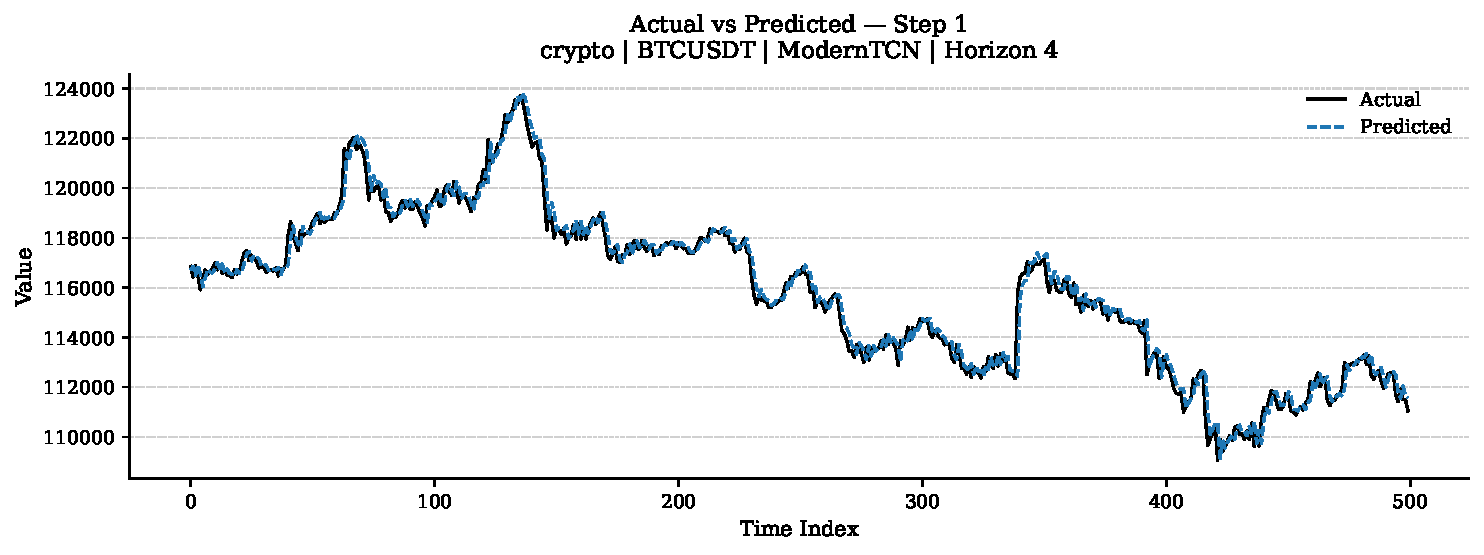
\includegraphics[width=\textwidth]{figures/08_predictions/crypto/ModernTCN/4/actual_vs_pred_step_1.pdf}
    \caption{Step~1 ($+$1 hour ahead).}
    \label{fig:pred_btc_h4_step1}
  \end{subfigure}
  \hfill
  \begin{subfigure}[b]{0.48\textwidth}
    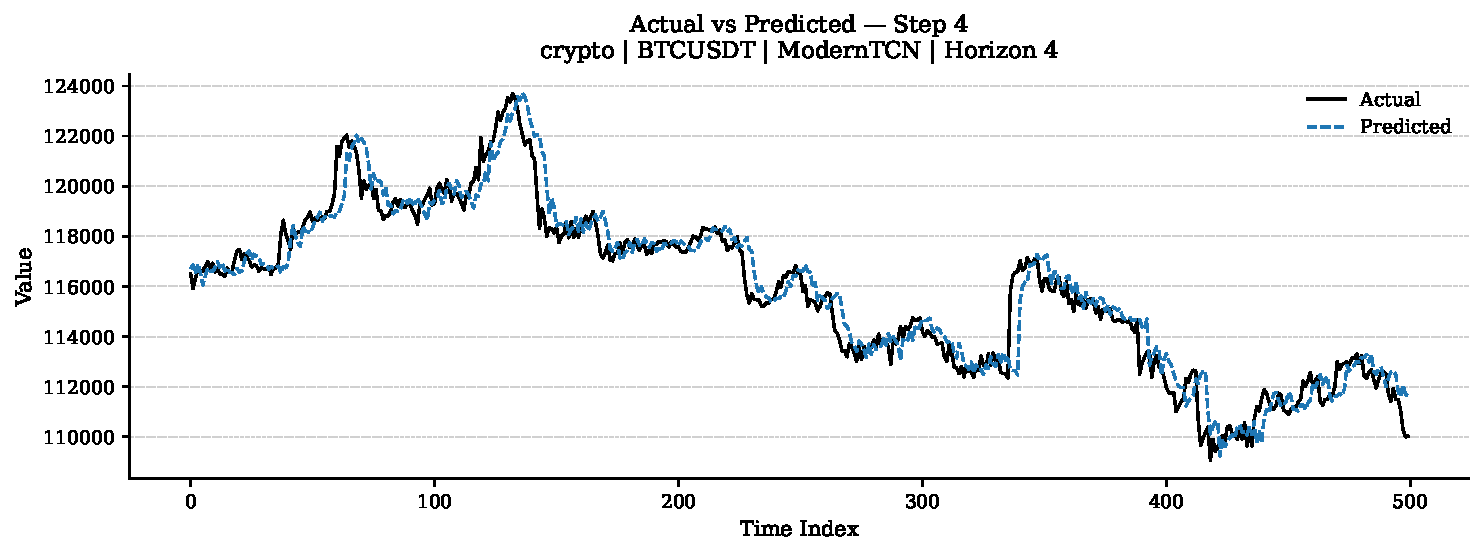
\includegraphics[width=\textwidth]{figures/08_predictions/crypto/ModernTCN/4/actual_vs_pred_step_4.pdf}
    \caption{Step~4 ($+$4 hours ahead).}
    \label{fig:pred_btc_h4_step4}
  \end{subfigure}
  \caption{Actual versus predicted close price for \moderntcn on BTC/USDT, $h = 4$ (seed~123).  (a)~At step~1, the model tracks the actual price with high fidelity, capturing directional turns and amplitude fluctuations.  (b)~At step~4, trend structure is preserved but short-lived volatility spikes are modestly attenuated, consistent with MSE-induced shrinkage.  No systematic phase shift is observed.}
  \label{fig:pred_btc_h4_step1_step4}
\end{figure}

Figure~\ref{fig:pred_short_contrast} juxtaposes \patchtst on EUR/USD and \timexer on Dow Jones, both at $\hfour$, step~1.  The EUR/USD panel (Figure~\ref{fig:pred_eurusd_patchtst_h4_step1}) shows that \patchtst's predictions follow the low-amplitude, mean-reverting dynamics of the currency pair with high precision, corroborating its category-leading \rmse in forex (0.1108; Table~\ref{tab:category_metrics}).  The Dow Jones panel (Figure~\ref{fig:pred_dji_timexer_h4_step1}) shows the middle-tier \timexer (rank~4): it tracks the general directional drift but exhibits a wider deviation band and less precise recovery of sharp reversals---a qualitative reflection of the rank gap between the top and middle tiers.

\begin{figure}[htbp]
  \centering
  \begin{subfigure}[b]{0.48\textwidth}
    
\includegraphics[width=\textwidth]{figures/08_predictions/forex/PatchTST/4/actual_vs_pred_step_1.pdf}
    \caption{\patchtst on EUR/USD, step~1 ($h = 4$).}
    \label{fig:pred_eurusd_patchtst_h4_step1}
  \end{subfigure}
  \hfill
  \begin{subfigure}[b]{0.48\textwidth}
    
\includegraphics[width=\textwidth]{figures/08_predictions/indices/TimeXer/4/actual_vs_pred_step_1.pdf}
    \caption{\timexer on Dow Jones, step~1 ($h = 4$).}
    \label{fig:pred_dji_timexer_h4_step1}
  \end{subfigure}
  \caption{Cross-architecture, cross-asset contrast at $h = 4$, step~1 (seed~123).  (a)~\patchtst on EUR/USD (rank~2) tracks the low-amplitude, mean-reverting forex dynamics with high accuracy.  (b)~\timexer on Dow Jones (rank~4) captures the directional structure but with a wider deviation band, illustrating the qualitative signature of the rank gap between top and middle tiers.}
  \label{fig:pred_short_contrast}
\end{figure}

Figure~\ref{fig:pred_itransformer_btc} provides a direct comparison between the third-ranked \itransformer and the top-ranked \moderntcn on BTC/USDT at $\hfour$.  Both models track the actual price trajectory closely at step~1, but at step~4 \itransformer exhibits slightly more amplitude attenuation during volatile episodes.  This visual difference is consistent with the small but consistent \rmse gap between \itransformer (743.5) and \moderntcn (731.6) on BTC/USDT at $\hfour$ (Table~\ref{tab:horizon_degradation_btc}).

\begin{figure}[htbp]
  \centering
  \begin{subfigure}[b]{0.48\textwidth}
    
\includegraphics[width=\textwidth]{figures/08_predictions/crypto/iTransformer/4/actual_vs_pred_step_1.pdf}
    \caption{\itransformer on BTC/USDT, step~1 ($h = 4$).}
    \label{fig:pred_btc_itransformer_h4_step1}
  \end{subfigure}
  \hfill
  \begin{subfigure}[b]{0.48\textwidth}
    
\includegraphics[width=\textwidth]{figures/08_predictions/crypto/iTransformer/4/actual_vs_pred_step_4.pdf}
    \caption{\itransformer on BTC/USDT, step~4 ($h = 4$).}
    \label{fig:pred_btc_itransformer_h4_step4}
  \end{subfigure}
  \caption{\itransformer (rank~3) on BTC/USDT at $\hfour$ (seed~123).  (a)~At step~1, tracking fidelity is comparable to \moderntcn (Figure~\ref{fig:pred_btc_h4_step1}).  (b)~At step~4, slightly more amplitude attenuation is visible relative to \moderntcn (Figure~\ref{fig:pred_btc_h4_step4}), consistent with the 1.6\% \rmse gap.  The inverted attention mechanism produces qualitatively similar but measurably weaker temporal representations for short-horizon cryptocurrency forecasting.}
  \label{fig:pred_itransformer_btc}
\end{figure}

% - - - - - - - - - - - - - - - - - - - - - - - - - - - - - - - - - - - - -
\paragraph{Medium-horizon behaviour ($h = 24$, step 12).}

Figure~\ref{fig:pred_medium_horizon} presents step-12 overlays from two model--asset pairings at the midpoint of the $\htwentyfour$ vector.  \moderntcn on EUR/USD (Figure~\ref{fig:pred_eurusd_moderntcn_h24_step12}) shows that macro-directional structure is preserved 12 hours ahead: the predicted series follows multi-session trends while understandably missing the sharpest intra-session swings.  \patchtst on Dow Jones (Figure~\ref{fig:pred_dji_patchtst_h24_step12}) similarly maintains directional integrity at step~12, but with a visibly wider error envelope than at $\hfour$---confirming the $2$--$2.5\times$ \rmse amplification (Table~\ref{tab:horizon_degradation_btc}).  Both panels show that the dominant degradation signature is amplitude attenuation rather than phase error or directional reversal.

\begin{figure}[htbp]
  \centering
  \begin{subfigure}[b]{0.48\textwidth}
    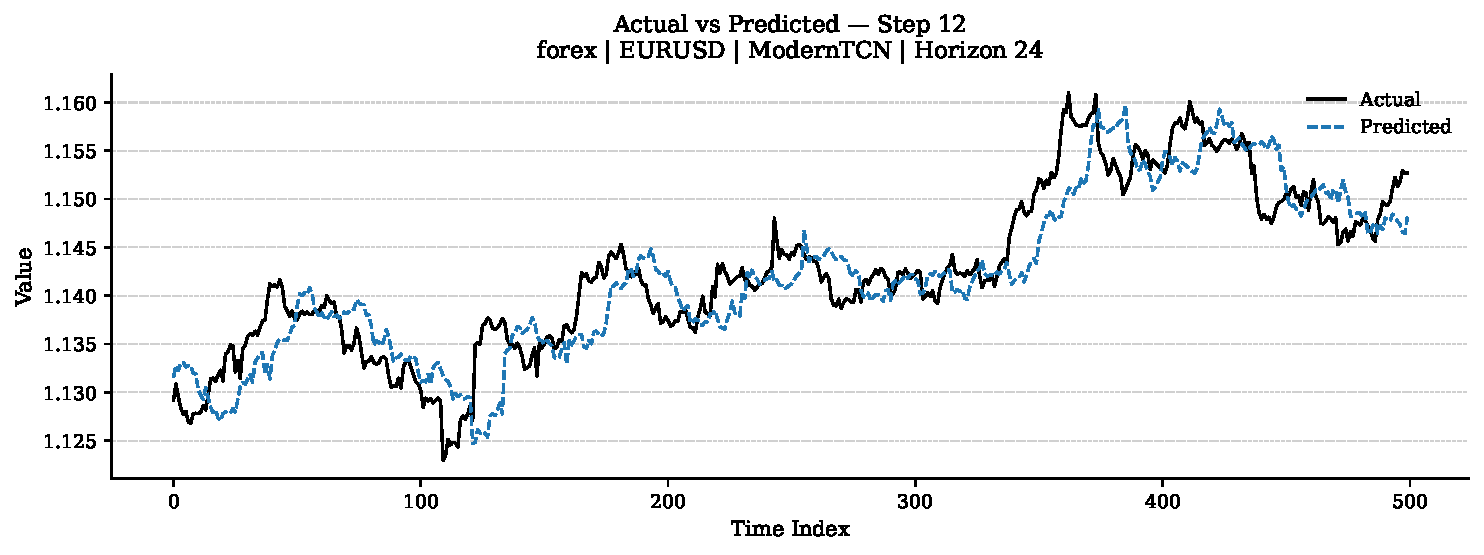
\includegraphics[width=\textwidth]{figures/08_predictions/forex/ModernTCN/24/actual_vs_pred_step_12.pdf}
    \caption{\moderntcn on EUR/USD, step~12 ($h = 24$).}
    \label{fig:pred_eurusd_moderntcn_h24_step12}
  \end{subfigure}
  \hfill
  \begin{subfigure}[b]{0.48\textwidth}
    
\includegraphics[width=\textwidth]{figures/08_predictions/indices/PatchTST/24/actual_vs_pred_step_12.pdf}
    \caption{\patchtst on Dow Jones, step~12 ($h = 24$).}
    \label{fig:pred_dji_patchtst_h24_step12}
  \end{subfigure}
  \caption{Medium-horizon actual-versus-predicted overlays at step~12 of the $h = 24$ forecast vector (seed~123).  (a)~\moderntcn on EUR/USD: directional content is preserved 12 hours ahead while high-frequency amplitude is dampened.  (b)~\patchtst on Dow Jones: directional integrity is maintained but the forecast envelope is wider than at $\hfour$, corroborating the $2$--$2.5\times$ \rmse amplification (Table~\ref{tab:horizon_degradation_btc}).  Both top architectures exhibit amplitude attenuation as the primary degradation mode.}
  \label{fig:pred_medium_horizon}
\end{figure}

% - - - - - - - - - - - - - - - - - - - - - - - - - - - - - - - - - - - - -
\paragraph{Long-horizon degradation ($h = 24$, step 24).}

Figure~\ref{fig:pred_long_horizon} presents the 24-step-ahead overlay for \moderntcn on BTC/USDT---the most demanding combination in the benchmark, pairing the highest price volatility with the maximum forecast depth.  The predicted series retains directional drift but shows progressive amplitude compression beyond step~12, with increasingly imprecise oscillatory reversal timing.  These characteristics are consistent with \moderntcn's \rmse degradation from 731.6 ($\hfour$) to 1{,}617.4 ($\htwentyfour$; Table~\ref{tab:horizon_degradation_btc})---a 121.1\% increase that, while substantial, does not erase directional signal or introduce systematic bias.  Long-horizon predictions are \emph{trend-indicative} rather than instance-specific: architectures differ not in whether degradation occurs but in how gracefully their temporal representations transfer to the maximum horizon.

\begin{figure}[htbp]
  \centering
  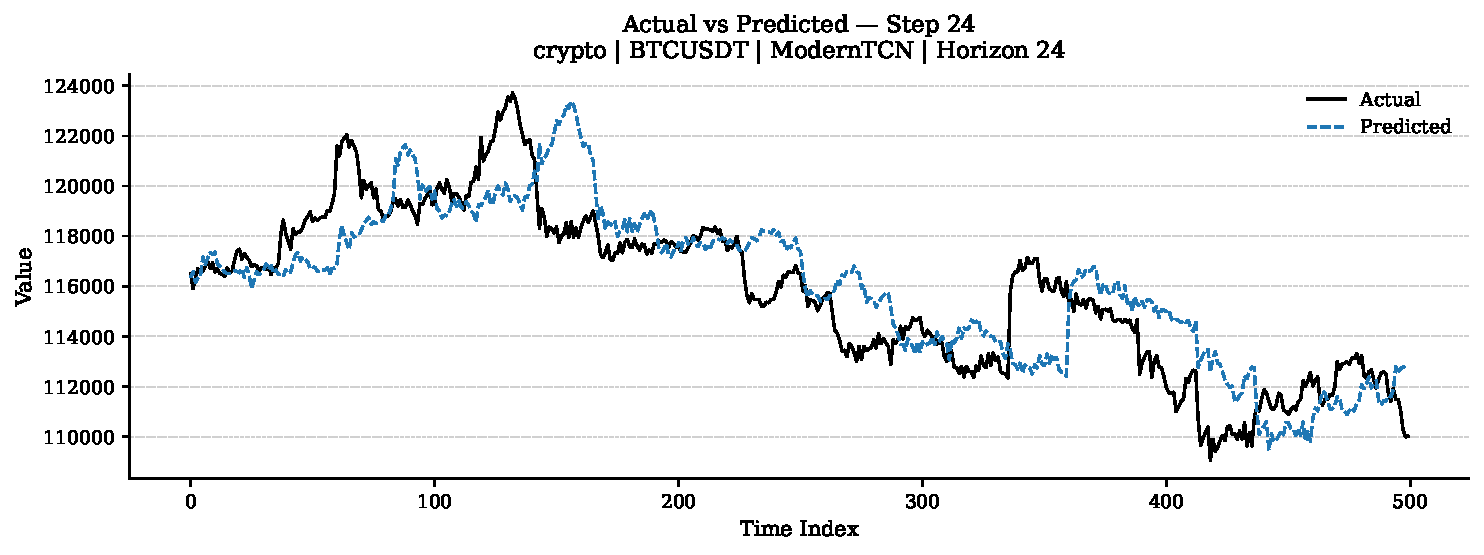
\includegraphics[width=0.80\textwidth]{figures/08_predictions/crypto/ModernTCN/24/actual_vs_pred_step_24.pdf}
  \caption{Long-horizon overlay: \moderntcn on BTC/USDT, $h = 24$, step~24 (seed~123).  The model retains directional integrity and captures low-frequency trend components, but high-amplitude intra-day reversals are under-predicted.  This pattern---directional fidelity without amplitude precision---is the signature of MSE-optimised direct multi-step forecasting at the maximum horizon.  The \rmse at $h = 24$ (1{,}617.4) represents a 121.1\% degradation relative to $\hfour$ (731.6; Table~\ref{tab:horizon_degradation_btc}).}
  \label{fig:pred_long_horizon}
\end{figure}
